% Manual paso a paso: construir y entrenar FuegoNet, una red tipo YOLO26 para
% detectar fuego y humo desde el Tarot 650. Compila con pdfLaTeX (por omisión en
% Overleaf), XeLaTeX o LuaLaTeX.
\documentclass[11pt,letterpaper,oneside,openany]{book}

\usepackage{iftex}
\ifPDFTeX
  \usepackage[utf8]{inputenc}
  \usepackage[T1]{fontenc}
  \usepackage{lmodern}
\else
  \usepackage{fontspec}
\fi
\usepackage[spanish,es-noshorthands,es-tabla]{babel}
\usepackage[margin=2.4cm]{geometry}
\usepackage{amsmath,amssymb}
\usepackage{graphicx}
\usepackage{booktabs,tabularx,array,longtable}
\usepackage{enumitem}
\usepackage[dvipsnames]{xcolor}
\usepackage[most]{tcolorbox}
\usepackage{listings}
\usepackage{tikz}
\usetikzlibrary{arrows.meta,positioning,shapes.geometric,shapes.misc,fit,calc,decorations.pathmorphing}
\usepackage{caption}
\usepackage{float}
\usepackage{xurl}
\usepackage[colorlinks=true,linkcolor=NavyBlue,urlcolor=NavyBlue,citecolor=NavyBlue]{hyperref}

\graphicspath{{figuras/}}
\setlist{itemsep=2pt,topsep=4pt}
\setlength{\parindent}{0pt}
\setlength{\parskip}{6pt}
\setlength{\emergencystretch}{3em}
\captionsetup{font=small,labelfont=bf}
\urlstyle{tt}

% Rutas, archivos, nodos y tópicos en monoespaciado (con _ y / sin escapar).
\newcommand{\cod}[1]{\expandafter\nolinkurl\expandafter{\detokenize{#1}}}
\newcommand{\sgn}{\operatorname{sgn}}
\newcommand{\Sgn}{\operatorname{Sgn}}

\lstset{basicstyle=\ttfamily\footnotesize,columns=fullflexible,keepspaces=true,breaklines=true,
        frame=single,rulecolor=\color{black!25},backgroundcolor=\color{black!3},
        xleftmargin=4pt,xrightmargin=4pt,aboveskip=6pt,belowskip=6pt,
        showstringspaces=false,upquote=true,
        literate={á}{{\'a}}1 {é}{{\'e}}1 {í}{{\'i}}1 {ó}{{\'o}}1 {ú}{{\'u}}1
                 {Á}{{\'A}}1 {É}{{\'E}}1 {Í}{{\'I}}1 {Ó}{{\'O}}1 {Ú}{{\'U}}1
                 {ñ}{{\~n}}1 {Ñ}{{\~N}}1 {ü}{{\"u}}1 {¿}{{?`}}1 {¡}{{!`}}1
                 {°}{{$^\circ$}}1 {²}{{$^2$}}1 {·}{{$\cdot$}}1 {→}{{$\rightarrow$}}1
                 {×}{{$\times$}}1 {±}{{$\pm$}}1 {—}{{---}}1 {–}{{--}}1
                 {«}{{\guillemotleft}}1 {»}{{\guillemotright}}1}
\lstdefinestyle{bash}{language=bash,morekeywords={ros2,colcon,source,sudo,git,gz,python3}}
\lstdefinestyle{py}{language=Python,keywordstyle=\color{NavyBlue}\bfseries,commentstyle=\color{black!55}\itshape,
                    stringstyle=\color{BrickRed}}
\lstdefinestyle{xml}{language=XML,keywordstyle=\color{NavyBlue},stringstyle=\color{BrickRed}}
\newcommand{\paso}[1]{\par\medskip\noindent\colorbox{NavyBlue!80!black}{\textcolor{white}{\bfseries\,Paso #1\,}}\enspace}

% Recuadros del libro.
\tcbset{enhanced,breakable,boxrule=0.6pt,arc=2pt,left=6pt,right=6pt,top=4pt,bottom=4pt,fonttitle=\bfseries}
\newtcolorbox{nota}{colback=NavyBlue!4,colframe=NavyBlue!70!black,title=Nota}
\newtcolorbox{aviso}{colback=BrickRed!5,colframe=BrickRed!70!black,title=Cuidado}
\newtcolorbox{leccion}{colback=ForestGreen!5,colframe=ForestGreen!70!black,title=Problema encontrado y cómo se resolvió}
\newtcolorbox{recuerda}{colback=Goldenrod!10,colframe=Goldenrod!80!black,title=Recuerda}
\newtcolorbox{consejo}{colback=Cyan!5,colframe=Cyan!60!black,title=Consejo}
\newtcolorbox{tecnico}{colback=black!3,colframe=black!45,title=Para curiosos (te lo puedes saltar)}
\newtcolorbox{ejemplo}[1][]{colback=Orchid!5,colframe=Orchid!70!black,title=Ejemplo de la vida diaria#1}
\newtcolorbox{ejercicio}{colback=Peach!8,colframe=Peach!80!black,title=Pruébalo tú}
\newtcolorbox{enpocas}{colback=ForestGreen!4,colframe=ForestGreen!50!black,title=En este capítulo}
\newtcolorbox{resultado}{colback=NavyBlue!3,colframe=NavyBlue!50!black,title=Lo que debes ver}

\title{\textbf{Tu propia red tipo YOLO26}\\[6pt]
\Large Manual paso a paso para construir y entrenar FuegoNet,\\
un detector de fuego y humo para el Tarot 650\\[10pt]
\large PyTorch · YOLO26 · ROS 2 Jazzy · Gazebo Harmonic}
\author{Dr.\ Jairo Olguín Roque\\
FES Acatlán, UNAM}
\date{Octubre de 2026}

\begin{document}
\frontmatter
\maketitle
\tableofcontents
\chapter*{Cómo usar este manual}
\addcontentsline{toc}{chapter}{Cómo usar este manual}

Este manual explica, paso a paso, cómo se construyó \textbf{FuegoNet}: una red
neuronal de detección de objetos con la misma arquitectura que YOLO26, escrita
desde cero en PyTorch, para reconocer \textbf{fuego} y \textbf{humo} en las
imágenes de la cámara del Tarot 650 durante la búsqueda de incendios forestales.

Hasta ahora la simulación usaba YOLO26n de Ultralytics: se descargan pesos
entrenados en COCO (80 clases de objetos cotidianos) y se ajustan a nuestras dos
clases. Funciona muy bien, pero la red es una caja negra: no se ve qué hace por
dentro, no se puede modificar con libertad y, en un trabajo de investigación, es difícil
justificar cada decisión. Aquí abrimos esa caja. Cada pieza de YOLO26 se
programa a mano, se prueba por separado y se explica con sus ecuaciones. Al final
se entrena la red completa \emph{sin pesos preentrenados} y se compara con
YOLO26n usando el mismo código de medición.

\section*{Qué necesitas saber antes}
\begin{itemize}
  \item Python básico (funciones, clases, listas) y saber correr un comando en la terminal.
  \item La idea de neurona, convolución, IoU y mAP. Si no la tienes, lee primero
        el capítulo «Redes neuronales y YOLO sin complicaciones» del libro de la
        simulación (\cod{doc/manual}). Aquí se repasa lo indispensable.
  \item No hace falta saber PyTorch: cada vez que aparece algo nuevo se explica.
\end{itemize}

\section*{Cómo está organizado}
\begin{description}
  \item[Parte I] Qué es YOLO26, qué tiene de nuevo y cómo preparar el entorno y los datos.
  \item[Parte II] Los bloques de la red (convoluciones, C3k2, SPPF, atención) y cómo se
        ensamblan en columna vertebral, cuello y cabeza.
  \item[Parte III] Cómo aprende: la asignación de etiquetas (TAL y STAL), la función
        de pérdida de dos cabezas, los aumentos de datos y el ciclo de entrenamiento
        con el optimizador MuSGD.
  \item[Parte IV] Cómo se mide, cómo se compara con YOLO26n y cómo se conecta a ROS 2
        para que el dron la use en vuelo.
\end{description}

Cada capítulo avanza en \textbf{pasos numerados}. Al final de cada paso hay un
recuadro «Lo que debes ver» con la salida esperada; si lo que ves es distinto,
no sigas: algo quedó mal en ese paso.

\section*{Convenciones}
\begin{itemize}
  \item Los comandos se escriben así y se corren desde \cod{~/ros2_ws/src/cuadrirotor_sim}:
\begin{lstlisting}[style=bash]
~/.venvs/yolo/bin/python -m cuadrirotor_sim.red_fuego.modelo
\end{lstlisting}
  \item Las rutas, archivos y nombres de variables van en \cod{monoespaciado}.
  \item El código completo está en \cod{cuadrirotor_sim/red_fuego/} y en el
        apéndice~\ref{ap:codigo}. En el texto solo aparecen las partes importantes.
  \item Los nombres del código están en español (\cod{Cuello}, \cod{Atencion},
        \cod{AsignadorTAL}) para que se lean junto con el texto. Entre paréntesis se
        da el nombre en inglés que vas a encontrar en los artículos.
\end{itemize}

\begin{nota}
Todos los números de este manual (parámetros, tiempos, mAP) salieron de correr el
código en la computadora del laboratorio: Ubuntu, PyTorch 2.14 con CUDA 13 y una
tarjeta NVIDIA RTX~5060~Ti de 16~GB. En otra máquina los tiempos cambian, pero
las métricas deben salir parecidas.
\end{nota}


\mainmatter
\part{Entender lo que vamos a construir}
\chapter{Qué es YOLO26 y qué vamos a copiar}
\label{cap:yolo26}

\begin{enpocas}
Qué hace un detector de una etapa, de dónde viene la familia YOLO y cuáles son
las cinco ideas de YOLO26 que vamos a programar: cabeza sin DFL, inferencia
sin NMS, ProgLoss, STAL y el optimizador MuSGD.
\end{enpocas}

\section{El problema: encontrar fuego y humo en una imagen}

La cámara del Tarot 650 entrega imágenes de $640\times480$ píxeles. Un
\textbf{detector de objetos} debe responder, para cada imagen, una lista de
\emph{cajas}: dónde está cada objeto (un rectángulo $x_1,y_1,x_2,y_2$), qué
es (fuego o humo) y qué tan seguro está (una confianza entre 0 y 1). La
misión de búsqueda (\cod{busqueda_incendio}) usa esas cajas para decidir hacia
dónde volar y cuándo confirmar el incendio.

\begin{ejemplo}
Piensa en un vigilante en una torre forestal. No le basta saber que «en algún
lado hay humo»: necesita señalar con el dedo \emph{dónde}, y distinguir una
columna de humo de una nube baja. Eso es la detección: clasificar \emph{y}
localizar.
\end{ejemplo}

\section{Detectores de una etapa: la idea de YOLO}

YOLO (\emph{You Only Look Once}, 2016) propuso mirar la imagen una sola vez.
La red reduce la imagen a una \textbf{rejilla} de celdas y cada celda predice,
en una sola pasada, si hay un objeto cerca de su centro, de qué clase es y
dónde están los bordes de su caja. No hay una etapa previa que proponga
regiones (como en Faster R-CNN), por eso es rápido y sirve en un dron.

Desde entonces la familia ha cambiado mucho. Para este manual importan tres pasos:
\begin{description}
  \item[YOLOv8 (2023)] Sin anclas predefinidas: cada celda predice distancias a los
        cuatro lados de la caja. Asignación de etiquetas \emph{alineada a la tarea}
        (TAL). Cada distancia se predice como una distribución sobre 16 valores
        (DFL, \emph{Distribution Focal Loss}).
  \item[YOLOv10 (2024)] Dos cabezas: una «uno a muchos» para entrenar y otra
        «uno a uno» para inferir. La segunda da una sola caja por objeto y
        elimina el NMS.
  \item[YOLO11 (2024)] Bloques C3k2 y atención espacial C2PSA en la columna vertebral.
\end{description}

\section{Lo nuevo de YOLO26}

YOLO26 (Ultralytics, 2025--2026) junta lo anterior y lo simplifica pensando en
equipos pequeños, como la computadora a bordo de un dron:

\begin{enumerate}
  \item \textbf{Sin DFL} (\cod{reg_max = 1}). Cada distancia es un solo número, no
        una distribución de 16. La cabeza es más pequeña, la exportación a ONNX
        o TensorRT es directa y la pérdida usa L1 en lugar de DFL.
  \item \textbf{Sin NMS, de extremo a extremo.} Usa la doble cabeza de YOLOv10. La
        salida ya trae una caja por objeto: basta ordenar por confianza.
  \item \textbf{ProgLoss.} El peso entre las dos cabezas cambia durante el entrenamiento:
        empieza dominando la de muchos positivos (aprende rápido) y termina dominando
        la de uno a uno (la que se usa al final).
  \item \textbf{STAL} (\emph{Small-Target-Aware Label assignment}). Las cajas muy pequeñas
        se agrandan al elegir celdas candidatas para que nunca se queden sin «responsable».
        A gran altura, un foco de fuego mide pocos píxeles: esto nos importa mucho.
  \item \textbf{MuSGD.} Un optimizador que mezcla SGD con Muon, un método nacido para
        entrenar modelos de lenguaje que «ortogonaliza» la actualización de cada
        matriz de pesos.
\end{enumerate}

\begin{nota}
Estas cinco ideas se tomaron leyendo el código fuente de Ultralytics 8.4
(archivos \cod{cfg/models/26/yolo26.yaml}, \cod{nn/modules/head.py},
\cod{utils/tal.py}, \cod{utils/loss.py} y \cod{optim/muon.py}). FuegoNet
reproduce la arquitectura y la receta de entrenamiento, pero su código es
independiente: no importa nada de Ultralytics.
\end{nota}

\section{El plan: FuegoNet}

FuegoNet copia la escala \textbf{n} (\emph{nano}) de YOLO26, la más pequeña y la
que ya usa la simulación. La tabla~\ref{tab:plan} resume qué se copia y dónde
está cada pieza.

\begin{table}[H]
\centering\small
\caption{Piezas de YOLO26 y su archivo en \cod{cuadrirotor_sim/red_fuego/}.}
\label{tab:plan}
\begin{tabularx}{\textwidth}{>{\raggedright}p{4.2cm}X>{\ttfamily}p{2.6cm}}
\toprule
\textbf{Pieza} & \textbf{Qué hace} & \textrm{\textbf{Archivo}}\\
\midrule
Conv, C3k2, SPPF, C2PSA & Bloques que extraen características & bloques.py\\
Columna, cuello y cabeza & La red completa, de la imagen a las cajas & modelo.py\\
TAL + STAL & Decide qué celdas responden por cada objeto & asignador.py\\
Pérdida E2E + ProgLoss & Mide el error de las dos cabezas & perdida.py\\
CIoU & Traslape de cajas para la pérdida & perdida\_iou.py\\
Mosaico, afín, HSV & Aumentos de datos & datos.py\\
MuSGD & Optimizador & optimizador.py\\
Ciclo de entrenamiento, EMA & Entrenar y guardar el mejor modelo & entrenar.py\\
mAP50, mAP50-95 & Medir & metricas.py, evaluar.py\\
Detector, ONNX & Usar la red & inferir.py, exportar.py\\
\bottomrule
\end{tabularx}
\end{table}

\begin{recuerda}
Que la arquitectura sea la misma no significa que los resultados lo sean. YOLO26n
de la simulación partió de pesos entrenados con 118\,000 imágenes de COCO;
FuegoNet empieza con pesos al azar y solo ve nuestras 5\,400 imágenes. Por eso,
en el capítulo~\ref{cap:evaluar} se compara además con un YOLO26n entrenado
\emph{también desde cero}: esa es la comparación justa que valida nuestro código.
\end{recuerda}

\chapter{Preparar el entorno y los datos}
\label{cap:preparar}

\begin{enpocas}
Comprobar que PyTorch ve la tarjeta gráfica, conocer el dataset de fuego y humo
que genera el simulador y crear la carpeta donde vivirá la red.
\end{enpocas}

\paso{1} \textbf{Comprobar el entorno de Python.}
La simulación ya tiene un entorno virtual para YOLO en \cod{~/.venvs/yolo}, con
PyTorch, OpenCV y Ultralytics. FuegoNet solo necesita PyTorch, OpenCV, NumPy y
PyYAML; Ultralytics se usa únicamente para comparar.

\begin{lstlisting}[style=bash]
~/.venvs/yolo/bin/python -c "import torch, cv2, numpy; \
  print(torch.__version__, torch.cuda.is_available(), torch.cuda.get_device_name(0)); \
  print(cv2.__version__, numpy.__version__)"
\end{lstlisting}

\begin{resultado}
\ttfamily\small 2.14.1+cu130 True NVIDIA GeForce RTX 5060 Ti\\
4.11.0 1.26.4
\end{resultado}

\begin{aviso}
NumPy debe ser de la serie 1.x en este entorno: el puente de ROS 2 Jazzy
(\cod{cv_bridge}, \cod{rclpy}) está compilado contra NumPy~1. Si instalas algo con
\cod{pip} y te sube NumPy a 2.x, regrésalo de inmediato:
\begin{lstlisting}[style=bash]
~/.venvs/yolo/bin/pip install "numpy==1.26.4" "ml-dtypes<0.6"
\end{lstlisting}
Nos pasó al instalar \cod{onnx}: pip subió NumPy a 2.5 sin avisar
(capítulo~\ref{cap:integrar}).
\end{aviso}

\paso{2} \textbf{Conocer el dataset.}
Las imágenes salen del propio simulador. \cod{scripts/capturar_dataset.py}
vuela el dron sobre los mundos \cod{bosque} y \cod{bosque_grande} con focos de
fuego en lugares al azar y escribe, para cada foto, un archivo de texto con las
cajas. Son dos datasets que se usan juntos:

\begin{table}[H]
\centering\small
\caption{Dataset de fuego y humo (imágenes de $640\times480$).}
\label{tab:dataset}
\begin{tabular}{llrrrr}
\toprule
\textbf{Dataset} & \textbf{Parte} & \textbf{Imágenes} & \textbf{Cajas fuego} & \textbf{Cajas humo} & \textbf{Sin objetos}\\
\midrule
\cod{incendio_bosque} & train & 2\,700 & 1\,927 & 2\,203 & 309\\
                      & val   &   300 &   213 &   239 &  40\\
\cod{incendio_bosque_grande} & train & 2\,700 & 891 & 1\,898 & 755\\
                      & val   &   300 &    98 &   213 &  81\\
\midrule
\textbf{Total} & train & 5\,400 & 2\,818 & 4\,101 & 1\,064\\
               & val   &   600 &   311 &   452 &   121\\
\bottomrule
\end{tabular}
\end{table}

Las imágenes «sin objetos» son importantes: le enseñan a la red que un claro
iluminado o una roca oscura \emph{no} son fuego (una roca dio falsos positivos al
principio; por eso se agregó el mundo grande).

El formato es el de YOLO. Cada imagen \cod{images/train/00001.jpg} tiene su
\cod{labels/train/00001.txt} con una línea por objeto:
\begin{lstlisting}
0 0.472461 0.706724 0.070710 0.106154
1 0.480463 0.596074 0.145035 0.212378
\end{lstlisting}
El primer número es la clase (0 = fuego, 1 = humo) y los otros cuatro son el
centro $(c_x, c_y)$, el ancho $w$ y el alto $h$ de la caja, \emph{divididos} entre
el ancho y el alto de la imagen (todo queda entre 0 y 1). Un archivo vacío
significa «no hay nada que detectar».

Los dos datasets se juntan con un \cod{data.yaml} que lista ambas carpetas:
\begin{lstlisting}
train:
  - /home/jairo/datasets/incendio_bosque/images/train
  - /home/jairo/datasets/incendio_bosque_grande/images/train
val:
  - /home/jairo/datasets/incendio_bosque/images/val
  - /home/jairo/datasets/incendio_bosque_grande/images/val
names:
  0: fuego
  1: humo
\end{lstlisting}
Está en \cod{~/datasets/combinado_incendio_bosque_incendio_bosque_grande/}
(lo creó \cod{scripts/entrenar_yolo.py}).

\begin{tecnico}
De las 6\,919 cajas de entrenamiento, 195 tienen un lado menor de 16 píxeles.
Son focos vistos desde lejos. Sin un cuidado especial (STAL,
capítulo~\ref{cap:asignacion}) esas cajas pueden quedar sin ninguna celda
que aprenda de ellas.
\end{tecnico}

\paso{3} \textbf{Crear la carpeta de la red.}
FuegoNet vive dentro del paquete de ROS 2 como un subpaquete de Python, para que
el nodo detector la pueda importar después:

\begin{lstlisting}[style=bash]
cd ~/ros2_ws/src/cuadrirotor_sim
mkdir -p cuadrirotor_sim/red_fuego
touch cuadrirotor_sim/red_fuego/__init__.py
\end{lstlisting}

Al terminar el manual la carpeta tendrá estos archivos:
\begin{lstlisting}
cuadrirotor_sim/red_fuego/
  __init__.py        bloques.py      modelo.py      asignador.py
  perdida_iou.py     perdida.py      datos.py       optimizador.py
  metricas.py        entrenar.py     evaluar.py     inferir.py
  exportar.py
\end{lstlisting}

Como son módulos de un paquete, se ejecutan con \cod{python -m} desde la
carpeta del paquete (así funcionan los \cod{import} relativos como
\cod{from .bloques import Conv}).


\part{Construir la red pieza por pieza}
\chapter{Los bloques de construcción}
\label{cap:bloques}

\begin{enpocas}
Las seis piezas con las que se arma YOLO26, cada una como una clase de PyTorch:
\cod{Conv}, \cod{Cuello}, \cod{C3k2}, \cod{SPPF}, \cod{Atencion} y \cod{C2PSA}.
Todo está en \cod{red_fuego/bloques.py}.
\end{enpocas}

\section{Cómo se escribe una capa en PyTorch}

En PyTorch toda capa es una clase que hereda de \cod{nn.Module}. En
\cod{__init__} se crean las sub-capas (las que tienen pesos) y en
\cod{forward} se dice qué se hace con la entrada. Los datos viajan como
\textbf{tensores} de cuatro dimensiones $(B, C, H, W)$: $B$ imágenes del lote,
$C$ canales y $H\times W$ píxeles. Una imagen RGB de $640\times640$ entra como
$(1, 3, 640, 640)$.

\section{Conv: la unidad mínima}

\paso{4} \textbf{Escribir \cod{Conv}.}
Toda convolución de YOLO va seguida de una normalización por lotes
(BatchNorm) y de la activación SiLU, $\mathrm{SiLU}(x) = x\,\sigma(x)$:

\begin{lstlisting}[style=py]
class Conv(nn.Module):
    def __init__(self, c1, c2, k=1, s=1, g=1, d=1, act=True):
        super().__init__()
        self.conv = nn.Conv2d(c1, c2, k, s, relleno(k, d), groups=g, dilation=d, bias=False)
        self.bn = nn.BatchNorm2d(c2, eps=1e-3, momentum=0.03)
        self.act = nn.SiLU(inplace=True) if act else nn.Identity()

    def forward(self, x):
        return self.act(self.bn(self.conv(x)))
\end{lstlisting}

\begin{itemize}
  \item \cod{c1}, \cod{c2}: canales de entrada y de salida. \cod{k}: tamaño del filtro.
  \item \cod{s}: paso (\emph{stride}). Con \cod{s=2} el mapa sale a la mitad de alto
        y de ancho: así es como la red «se aleja» de la imagen.
  \item \cod{relleno(k)} $=\lfloor k/2\rfloor$ conserva el tamaño cuando \cod{s=1}.
  \item No lleva sesgo (\cod{bias=False}) porque BatchNorm ya suma uno.
  \item \cod{g} (grupos) permite la convolución \emph{en profundidad}
        (\cod{DWConv}): cada canal tiene su propio filtro y no se mezcla con los demás.
        Cuesta $C$ veces menos y la usa la cabeza de clases.
\end{itemize}

Una \cod{Conv} $3\times3$ de 64 a 128 canales tiene $64\cdot128\cdot9 = 73\,728$
pesos más $2\cdot128$ de BatchNorm: $73\,984$ parámetros.

\section{Cuello (bottleneck) y C3k}

\paso{5} \textbf{Escribir el cuello de botella residual.}
Dos \cod{Conv} $3\times3$ y un atajo que suma la entrada:
$\mathbf{y} = \mathbf{x} + f(\mathbf{x})$. El atajo deja pasar el gradiente sin
obstáculos y permite apilar muchas capas (la idea de ResNet).

\begin{lstlisting}[style=py]
class Cuello(nn.Module):
    def __init__(self, c1, c2, atajo=True, k=(3, 3), e=0.5):
        super().__init__()
        c_ = int(c2 * e)
        self.cv1 = Conv(c1, c_, k[0])
        self.cv2 = Conv(c_, c2, k[1])
        self.suma = atajo and c1 == c2

    def forward(self, x):
        y = self.cv2(self.cv1(x))
        return x + y if self.suma else y
\end{lstlisting}

\cod{C3k} es un CSP (\emph{Cross Stage Partial}) de tres convoluciones: la
entrada se proyecta por dos caminos; uno pasa por dos cuellos y el otro no; al
final se concatenan. Es más rico que un cuello solo y lo usan las etapas
profundas.

\section{C3k2: el bloque principal}

\paso{6} \textbf{Escribir \cod{C3k2}.}
Es el bloque que más se repite en YOLO26 (8 de las 23 capas). La
figura~\ref{fig:c3k2} muestra su flujo:

\begin{figure}[H]
\centering
\begin{tikzpicture}[font=\small,>=Stealth,
  caja/.style={draw,rounded corners=2pt,minimum height=7mm,minimum width=14mm,fill=NavyBlue!8},
  op/.style={draw,circle,inner sep=1pt,fill=Goldenrod!20}]
\node[caja] (in) {entrada $c_1$};
\node[caja,right=6mm of in] (cv1) {Conv $1{\times}1$};
\node[op,right=6mm of cv1] (sp) {$\div 2$};
\node[caja,right=8mm of sp,yshift=-9mm] (m1) {sub 1};
\node[caja,right=6mm of m1] (m2) {sub 2};
\node[right=3mm of m2] (pts) {$\cdots$};
\node[op,right=30mm of sp,yshift=9mm] (cat) {C};
\node[caja,right=6mm of cat] (cv2) {Conv $1{\times}1$};
\node[caja,right=6mm of cv2] (out) {salida $c_2$};
\draw[->] (in)--(cv1); \draw[->] (cv1)--(sp);
\draw[->] (sp) |- node[pos=0.75,above]{$c$} (cat);
\draw[->] (sp) |- node[pos=0.75,below]{$c$} (m1);
\draw[->] (m1)--(m2); \draw[->] (m2)--(pts);
\draw[->] (m1.north) -- ++(0,4mm) -| ([xshift=-1mm]cat.south);
\draw[->] (m2.north) -- ++(0,2mm) -| ([xshift=1mm]cat.south);
\draw[->] (cat)--node[above]{$(2{+}n)c$}(cv2); \draw[->] (cv2)--(out);
\end{tikzpicture}
\caption{C3k2. La entrada se proyecta a $2c$ canales y se parte en dos. La
segunda mitad pasa por $n$ subbloques en cadena; \emph{todas} las salidas
intermedias se concatenan (C) y una Conv $1{\times}1$ las mezcla. El subbloque
es un \cod{Cuello}, un \cod{C3k} o un \cod{Cuello} + atención.}
\label{fig:c3k2}
\end{figure}

\begin{lstlisting}[style=py]
class C3k2(nn.Module):
    def __init__(self, c1, c2, n=1, c3k=False, e=0.5, atencion=False, atajo=True):
        super().__init__()
        self.c = int(c2 * e)
        self.cv1 = Conv(c1, 2 * self.c, 1)
        self.cv2 = Conv((2 + n) * self.c, c2, 1)
        if atencion:
            sub = lambda: nn.Sequential(Cuello(self.c, self.c, atajo),
                                        BloquePSA(self.c, cabezas=max(self.c // 64, 1)))
        elif c3k:
            sub = lambda: C3k(self.c, self.c, 2, atajo)
        else:
            sub = lambda: Cuello(self.c, self.c, atajo)
        self.m = nn.ModuleList(sub() for _ in range(n))

    def forward(self, x):
        y = list(self.cv1(x).chunk(2, 1))      # dos mitades de c canales
        for m in self.m:
            y.append(m(y[-1]))                  # cada subbloque toma la última salida
        return self.cv2(torch.cat(y, 1))
\end{lstlisting}

\begin{consejo}
El parámetro \cod{e} (expansión) controla el ancho interno. YOLO26 usa
\cod{e=0.25} en las dos primeras etapas (mapas grandes, conviene ahorrar
cómputo) y \cod{e=0.5} en las demás.
\end{consejo}

\section{SPPF: ver a varias escalas}

\paso{7} \textbf{Escribir \cod{SPPF}.}
Al final de la columna vertebral el mapa mide $20\times20$. Para que cada celda
vea su contexto (¿esa mancha naranja está junto a una columna de humo?),
\cod{SPPF} aplica tres \emph{max-pool} de $5\times5$ en cadena. Tres
ventanas de 5 equivalen a ventanas de 5, 9 y 13 celdas, sin agregar ningún
parámetro. Las cuatro versiones se concatenan y se mezclan; YOLO26 agrega
además un atajo $\mathbf{y} \leftarrow \mathbf{y} + \mathbf{x}$.

\begin{lstlisting}[style=py]
    def forward(self, x):
        y = [self.cv1(x)]
        for _ in range(self.n):              # n = 3
            y.append(self.m(y[-1]))          # MaxPool2d(5, 1, 2)
        y = self.cv2(torch.cat(y, 1))
        return x + y if self.suma else y
\end{lstlisting}

\section{Atención: que cada celda mire a todas las demás}

\paso{8} \textbf{Escribir \cod{Atencion}, \cod{BloquePSA} y \cod{C2PSA}.}
Una convolución solo mira a sus vecinos. La \textbf{autoatención} deja que cada
celda consulte a \emph{todas} las demás. Si el mapa tiene $N = H\,W$ celdas, de
cada una se calculan tres vectores con convoluciones $1\times1$: una
\emph{consulta} $\mathbf{q}_i$, una \emph{llave} $\mathbf{k}_j$ y un
\emph{valor} $\mathbf{v}_j$. La salida de la celda $i$ es un promedio pesado de
los valores:
\begin{equation}
\mathbf{y}_i = \sum_{j=1}^{N} a_{ij}\,\mathbf{v}_j,\qquad
a_{ij} = \frac{\exp(\mathbf{q}_i\cdot\mathbf{k}_j/\sqrt{d_k})}
              {\sum_{l}\exp(\mathbf{q}_i\cdot\mathbf{k}_l/\sqrt{d_k})}.
\end{equation}
El peso $a_{ij}$ es grande cuando la consulta de $i$ «se parece» a la llave de
$j$. Con varias \emph{cabezas} se hacen varias atenciones en paralelo, cada una
con su parte de los canales. Se suma además una convolución $3\times3$ en
profundidad sobre $\mathbf{v}$, que le dice a la red dónde está cada celda
(codificación posicional).

\begin{lstlisting}[style=py]
    def forward(self, x):
        B, C, H, W = x.shape
        q, k, v = self.qkv(x).view(B, self.cabezas, 2 * self.dk + self.dc, H * W).split(
            [self.dk, self.dk, self.dc], dim=2)
        a = ((q * self.escala).transpose(-2, -1) @ k).softmax(dim=-1)   # (B, h, N, N)
        y = (v @ a.transpose(-2, -1)).view(B, C, H, W) + self.pe(v.reshape(B, C, H, W))
        return self.proy(y)
\end{lstlisting}

\begin{aviso}
La matriz $a$ tiene $N\times N$ elementos. Con el mapa de $20\times20$ son
$400^2 = 160\,000$ por cabeza: barato. Con el de $80\times80$ serían
$41$ millones. Por eso YOLO26 solo pone atención en la etapa más profunda
($P_5$).
\end{aviso}

\cod{BloquePSA} es como un bloque de transformador: atención con atajo y luego
una pequeña red de avance (dos Conv $1\times1$) también con atajo.
\cod{C2PSA} aplica la atención solo a la mitad de los canales (estilo CSP) y la
otra mitad pasa directo.

\paso{9} \textbf{Probar cada bloque.}
Antes de ensamblar nada hay que comprobar que cada bloque recibe y entrega las
formas correctas:
\begin{lstlisting}[style=py]
import torch
from cuadrirotor_sim.red_fuego.bloques import Conv, Cuello, C3k2, SPPF, C2PSA
x = torch.randn(1, 64, 80, 80)
for nombre, b in [('Conv 3x3 s=2', Conv(64, 128, 3, 2)), ('Cuello', Cuello(64, 64)),
                  ('C3k2 n=1', C3k2(64, 128, 1, False, 0.25)), ('C3k2 c3k', C3k2(64, 128, 1, True)),
                  ('SPPF', SPPF(64, 64, atajo=True)), ('C2PSA', C2PSA(64, 64))]:
    y = b(x)
    print(nombre, tuple(x.shape), '->', tuple(y.shape), sum(p.numel() for p in b.parameters()))
\end{lstlisting}

\begin{resultado}
\begin{lstlisting}
Conv 3x3 s=2   (1, 64, 80, 80) -> (1, 128, 40, 40)   73984 parámetros
Cuello         (1, 64, 80, 80) -> (1, 64, 80, 80)   37056 parámetros
C3k2 n=1       (1, 64, 80, 80) -> (1, 128, 80, 80)   26080 parámetros
C3k2 c3k       (1, 64, 80, 80) -> (1, 128, 80, 80)   78848 parámetros
SPPF           (1, 64, 80, 80) -> (1, 64, 80, 80)   10432 parámetros
C2PSA          (1, 64, 80, 80) -> (1, 64, 80, 80)   16352 parámetros
\end{lstlisting}
\end{resultado}

\begin{ejercicio}
Cambia \cod{e=0.25} por \cod{e=0.5} en el \cod{C3k2 n=1} y vuelve a contar los
parámetros. ¿Por qué crecen casi cuatro veces si solo duplicaste el ancho?
(Pista: en una convolución los pesos son $c_{\text{in}}\cdot c_{\text{out}}\cdot k^2$.)
\end{ejercicio}

\chapter{Ensamblar la red: columna, cuello y cabeza}
\label{cap:arquitectura}

\begin{enpocas}
Cómo se apilan los bloques para formar FuegoNet-n, cómo la cabeza convierte
mapas de características en cajas y por qué la salida ya no necesita NMS. Todo
está en \cod{red_fuego/modelo.py}.
\end{enpocas}

\section{La forma general}

Un detector moderno tiene tres partes (figura~\ref{fig:arquitectura}):
\begin{description}
  \item[Columna vertebral (\emph{backbone})] reduce la imagen paso a paso
        (a 1/2, 1/4, 1/8, 1/16 y 1/32) y aumenta los canales. Los mapas
        pequeños «saben» mucho (contexto) pero ven con poco detalle.
  \item[Cuello (\emph{neck}, PAN-FPN)] mezcla las escalas: primero de arriba abajo
        (el contexto de $P_5$ baja a $P_4$ y $P_3$) y luego de abajo arriba (el
        detalle de $P_3$ sube a $P_4$ y $P_5$).
  \item[Cabeza (\emph{head})] en cada celda de las tres escalas predice 4 distancias
        y 2 puntuaciones de clase.
\end{description}

\begin{figure}[H]
\centering
\begin{tikzpicture}[font=\scriptsize,>=Stealth,
  b/.style={draw,rounded corners=2pt,minimum width=26mm,minimum height=5.5mm,fill=NavyBlue!8,align=center},
  n/.style={b,minimum width=25mm,fill=ForestGreen!10},
  h/.style={b,minimum width=21mm,minimum height=8mm,fill=BrickRed!10}]
\foreach \t [count=\i from 0] in {Imagen $640^2{\times}3$, Conv s2 \;$320^2{\times}16$,
  Conv s2 \;$160^2{\times}32$, C3k2 \;$160^2{\times}64$, Conv s2 \;$80^2{\times}64$,
  C3k2 \;$80^2{\times}128$, Conv s2 \;$40^2{\times}128$, C3k2 \;$40^2{\times}128$,
  Conv s2 \;$20^2{\times}256$, C3k2 \;$20^2{\times}256$, SPPF \;$20^2{\times}256$,
  C2PSA \;$20^2{\times}256$}
  \node[b] (b\i) at (0,-0.8*\i) {\t};
\foreach \i [evaluate=\i as \j using int(\i+1)] in {0,...,10} \draw[->] (b\i)--(b\j);
% cuello: de arriba abajo (x = 4.6) y de abajo arriba (x = 8.2)
\node[n] (h16) at (4.6,-4.0) {C3k2 \;$80^2{\times}64$};
\node[n] (h13) at (4.6,-5.6) {C3k2 \;$40^2{\times}128$};
\node[n] (h19) at (8.2,-5.6) {C3k2 \;$40^2{\times}128$};
\node[n] (h22) at (8.2,-8.8) {C3k2+atn \;$20^2{\times}256$};
% cabeza
\node[h] (d3) at (11.8,-4.0) {cabeza $P_3$\\ $80^2$ celdas, paso 8};
\node[h] (d4) at (11.8,-5.6) {cabeza $P_4$\\ $40^2$ celdas, paso 16};
\node[h] (d5) at (11.8,-8.8) {cabeza $P_5$\\ $20^2$ celdas, paso 32};
\node[h,fill=Goldenrod!15] (sal) at (11.8,-10.4) {8\,400 celdas $\rightarrow$\\ 300 de mayor confianza};
% conexiones
\draw[->] (b5.east) -- (h16.west);
\draw[->] (b7.east) -- (h13.west);
\draw[->] (b11.east) -- (h22.west);
\draw[->] ([xshift=-6mm]h13.south |- b11.east) -- node[pos=0.5,left]{sube $\times2$} ([xshift=-6mm]h13.south);
\draw[->] ([xshift=-6mm]h13.north) -- node[left]{sube $\times2$} ([xshift=-6mm]h16.south);
\draw[->] ([xshift=6mm]h16.south) -- ++(0,-0.35) -| node[pos=0.25,above]{Conv s2} ([xshift=-6mm]h19.north);
\draw[->] (h13.east) -- (h19.west);
\draw[->] (h19.south) -- node[right]{Conv s2} (h22.north);
\draw[->] (h16.east) -- (d3.west);
\draw[->] (h19.east) -- (d4.west);
\draw[->] (h22.east) -- (d5.west);
\draw[->] (d5.south) -- (sal.north);
\node[text=NavyBlue,font=\small\bfseries] at (0,0.7) {columna vertebral};
\node[text=ForestGreen!60!black,font=\small\bfseries] at (6.4,-3.1) {cuello (PAN-FPN)};
\node[text=BrickRed,font=\small\bfseries] at (11.8,-3.1) {cabeza};
\end{tikzpicture}
\caption{FuegoNet-n con una imagen de $640\times640$. Cada caja muestra el tamaño
del mapa (alto$\times$ancho$\times$canales). Las flechas al cuello son
concatenaciones.}
\label{fig:arquitectura}
\end{figure}

\section{Escalas: n, s y m}

YOLO26 define cada tamaño con dos números: un factor de profundidad (cuántas
veces se repite cada bloque) y uno de anchura (cuántos canales). El archivo
\cod{yolo26.yaml} escribe la red con los canales de la versión grande y se
multiplican:

\begin{lstlisting}[style=py]
ESCALAS = {'n': (0.50, 0.25, 1024), 's': (0.50, 0.50, 1024), 'm': (0.50, 1.00, 512)}
...
c = lambda x: int(math.ceil(min(x, cmax) * anch / 8) * 8)   # canales múltiplos de 8
n = lambda x: max(round(x * prof), 1)                        # repeticiones
\end{lstlisting}

Así, la capa que en el \emph{yaml} tiene 1\,024 canales queda con
$1024\cdot0.25 = 256$ en la versión \textbf{n}.

\section{La columna vertebral y el cuello}

\paso{10} \textbf{Escribir \cod{FuegoNet.__init__}.}
Se copian las 23 capas de \cod{yolo26.yaml} en el mismo orden. Los nombres
\cod{b0}--\cod{b10} y \cod{h13}--\cod{h22} conservan el número de capa del
\emph{yaml} para poder compararlos:

\begin{lstlisting}[style=py]
        self.b0 = Conv(3, c(64), 3, 2)                                   # P1/2
        self.b1 = Conv(c(64), c(128), 3, 2)                              # P2/4
        self.b2 = C3k2(c(128), c(256), n(2), c3k, 0.25)
        self.b3 = Conv(c(256), c(256), 3, 2)                             # P3/8
        self.b4 = C3k2(c(256), c(512), n(2), c3k, 0.25)                  # -> P3
        self.b5 = Conv(c(512), c(512), 3, 2)                             # P4/16
        self.b6 = C3k2(c(512), c(512), n(2), True)                       # -> P4
        self.b7 = Conv(c(512), c(1024), 3, 2)                            # P5/32
        self.b8 = C3k2(c(1024), c(1024), n(2), True)
        self.b9 = SPPF(c(1024), c(1024), 5, 3, atajo=True)
        self.b10 = C2PSA(c(1024), c(1024), n(2))                         # -> P5
        self.sube = nn.Upsample(None, 2, 'nearest')
        self.h13 = C3k2(c(1024) + c(512), c(512), n(2), True)
        self.h16 = C3k2(c(512) + c(512), c(256), n(2), True)             # salida P3
        self.h17 = Conv(c(256), c(256), 3, 2)
        self.h19 = C3k2(c(256) + c(512), c(512), n(2), True)             # salida P4
        self.h20 = Conv(c(512), c(512), 3, 2)
        self.h22 = C3k2(c(512) + c(1024), c(1024), 1, True, 0.5, atencion=True)  # P5
        self.cabeza = Cabeza(nc, (c(256), c(512), c(1024)))
\end{lstlisting}

\paso{11} \textbf{Escribir \cod{FuegoNet.forward}.}
El recorrido se lee de arriba abajo como la figura:
\begin{lstlisting}[style=py]
    def forward(self, x):
        x = self.b2(self.b1(self.b0(x)))
        p3 = self.b4(self.b3(x))
        p4 = self.b6(self.b5(p3))
        p5 = self.b10(self.b9(self.b8(self.b7(p4))))
        t4 = self.h13(torch.cat((self.sube(p5), p4), 1))     # de arriba abajo
        s3 = self.h16(torch.cat((self.sube(t4), p3), 1))
        s4 = self.h19(torch.cat((self.h17(s3), t4), 1))      # de abajo arriba
        s5 = self.h22(torch.cat((self.h20(s4), p5), 1))
        return self.cabeza([s3, s4, s5])
\end{lstlisting}

\begin{table}[H]
\centering\small
\caption{FuegoNet-n capa por capa (entrada $640\times640$, 2 clases).}
\label{tab:capas}
\begin{tabular}{rlllr}
\toprule
\textbf{Capa} & \textbf{Bloque} & \textbf{Entra de} & \textbf{Salida} & \textbf{Parámetros}\\
\midrule
0 & Conv $3{\times}3$ s2 & imagen & $320\times320\times16$ & 464\\
1 & Conv $3{\times}3$ s2 & 0 & $160\times160\times32$ & 4\,672\\
2 & C3k2 ($e=0.25$) & 1 & $160\times160\times64$ & 6\,640\\
3 & Conv $3{\times}3$ s2 & 2 & $80\times80\times64$ & 36\,992\\
4 & C3k2 ($e=0.25$) & 3 & $80\times80\times128$ & 26\,080\\
5 & Conv $3{\times}3$ s2 & 4 & $40\times40\times128$ & 147\,712\\
6 & C3k2 (C3k) & 5 & $40\times40\times128$ & 87\,040\\
7 & Conv $3{\times}3$ s2 & 6 & $20\times20\times256$ & 295\,424\\
8 & C3k2 (C3k) & 7 & $20\times20\times256$ & 346\,112\\
9 & SPPF & 8 & $20\times20\times256$ & 164\,608\\
10 & C2PSA & 9 & $20\times20\times256$ & 249\,728\\
13 & C3k2 & sube(10) + 6 & $40\times40\times128$ & 119\,808\\
16 & C3k2 & sube(13) + 4 & $80\times80\times64$ & 34\,304\\
17 & Conv $3{\times}3$ s2 & 16 & $40\times40\times64$ & 36\,992\\
19 & C3k2 & 17 + 13 & $40\times40\times128$ & 95\,232\\
20 & Conv $3{\times}3$ s2 & 19 & $20\times20\times128$ & 147\,712\\
22 & C3k2 + atención & 20 + 10 & $20\times20\times256$ & 463\,104\\
23 & Cabeza (o2m + o2o) & 16, 19, 22 & $300\times6$ & 241\,956\\
\midrule
& \textbf{Total} & & & \textbf{2\,504\,580}\\
\bottomrule
\end{tabular}
\end{table}

\section{La cabeza: de mapas a cajas}

Las tres salidas del cuello tienen $80^2 + 40^2 + 20^2 = 8\,400$ celdas. Cada
celda tiene un centro $(a_x, a_y)$ y un \textbf{paso} $s$ (8, 16 o 32 píxeles):
el tamaño que ocupa en la imagen original. La cabeza predice para cada celda:
\begin{itemize}
  \item 4 distancias $(\ell, t, r, b)$ en unidades de celda, del centro a los lados
        izquierdo, superior, derecho e inferior de la caja;
  \item 2 \emph{logits}, uno por clase; la probabilidad es $\sigma(\text{logit})$.
\end{itemize}
La caja en píxeles es
\begin{equation}
x_1 = s\,(a_x - \ell),\quad y_1 = s\,(a_y - t),\quad
x_2 = s\,(a_x + r),\quad y_2 = s\,(a_y + b).
\label{eq:caja}
\end{equation}

\begin{tecnico}
YOLOv8 y YOLO11 predicen cada distancia como una distribución de probabilidad
sobre 16 valores enteros (DFL) y toman su media. YOLO26 la quita
(\cod{reg_max = 1}): la capa final da 4 números en lugar de 64. El error de
las distancias se mide con L1 (capítulo~\ref{cap:perdida}).
\end{tecnico}

\paso{12} \textbf{Escribir la clase \cod{Cabeza}.}
Hay dos ramas por escala: la de cajas (dos Conv $3\times3$ y una $1\times1$ que
da 4 canales) y la de clases (convoluciones en profundidad, más ligeras). Y todo
esto aparece \textbf{dos veces}: la cabeza «uno a muchos» (o2m) y su copia «uno
a uno» (o2o).

\begin{lstlisting}[style=py]
    def forward(self, x):
        if not self.training:   # al inferir solo se usa la o2o: la o2m ni se calcula
            return self.decodificar(self._ramas(x, self.caja_o2o, self.clase_o2o))
        o2m = self._ramas(x, self.caja, self.clase)
        # La o2o ve las características desconectadas del grafo: su gradiente
        # no modifica la columna vertebral (la entrena solo la rama o2m).
        o2o = self._ramas([xi.detach() for xi in x], self.caja_o2o, self.clase_o2o)
        return {'o2m': o2m, 'o2o': o2o}
\end{lstlisting}

En entrenamiento se devuelven las dos ramas para calcular la pérdida. En
inferencia solo se calcula la o2o y se decodifica (la o2m queda como peso muerto):

\begin{lstlisting}[style=py]
    def decodificar(self, p):
        puntos, paso = anclas(p['mapas'], self.pasos)
        cajas = dist_a_caja(p['dist'], puntos) * paso          # ecuación de la caja
        conf, clase = p['logits'].sigmoid().max(-1)
        conf, idx = conf.topk(min(self.max_det, conf.shape[1]), dim=1)
        ...
        return torch.cat((cajas, conf[..., None], clase[..., None]), -1)  # (B, 300, 6)
\end{lstlisting}

\section{¿Por qué ya no hace falta NMS?}

Con la asignación clásica, varias celdas vecinas aprenden a detectar el mismo
foco de fuego y todas dan una caja parecida. Hay que borrar los duplicados con
\textbf{NMS} (\emph{Non-Maximum Suppression}): ordenar por confianza y quitar las
cajas que traslapan mucho con una mejor. El NMS es un ciclo con condiciones que
no se paraleliza bien, su costo depende del número de cajas y complica exportar
la red.

La cabeza o2o se entrena de modo que \emph{solo una celda} por objeto tenga
confianza alta (capítulo~\ref{cap:asignacion}). A la salida basta tomar las 300
puntuaciones más altas y aplicar un umbral. La salida tiene siempre la misma
forma $(B, 300, 6)$ y el grafo exportado a ONNX termina ahí.

\paso{13} \textbf{Probar la red completa.}
\begin{lstlisting}[style=bash]
~/.venvs/yolo/bin/python -m cuadrirotor_sim.red_fuego.modelo
\end{lstlisting}
\begin{resultado}
\begin{lstlisting}
FuegoNet-n: 2.50 M parámetros, salida (1, 300, 6)
FuegoNet-s: 9.95 M parámetros, salida (1, 300, 6)
FuegoNet-m: 21.78 M parámetros, salida (1, 300, 6)
\end{lstlisting}
El YOLO26n ajustado de la simulación tiene 2.53~M parámetros. La diferencia
(1.3\,\%) viene de detalles menores de la cabeza. La arquitectura es la misma.
\end{resultado}

\begin{nota}
La inicialización importa. \cod{iniciar_sesgos} pone el sesgo de la última capa
de clases en $\log\!\big(5 / (n_c\,(640/s)^2)\big)$, una probabilidad inicial de
alrededor de 0.0001 por celda: al principio la red cree que \emph{todo} es fondo,
que es lo correcto en el 99.9\,\% de las celdas. Sin esto, la pérdida de clase de
las primeras iteraciones es enorme y el entrenamiento se vuelve inestable.
\end{nota}


\part{Enseñarle a la red}
\chapter{Quién responde por cada objeto: TAL y STAL}
\label{cap:asignacion}

\begin{enpocas}
Antes de calcular el error hay que decidir qué celdas \emph{deberían} haber
detectado cada foco de fuego y cuáles son fondo. Esa decisión, la
\textbf{asignación de etiquetas}, es lo que distingue a un detector de otro. Aquí se
programa la de YOLO26: TAL con dos variantes (uno a muchos y uno a uno) y el
ajuste STAL para objetos diminutos. Archivo: \cod{red_fuego/asignador.py}.
\end{enpocas}

\section{El problema}

Una imagen produce 8\,400 predicciones y tiene, digamos, una caja de fuego y una
de humo. ¿Contra qué etiqueta comparamos cada predicción? Si a todas las celdas
dentro de la caja les exigimos «fuego», las del borde (que apenas ven llamas)
reciben un objetivo imposible. Si solo a la del centro, la red recibe muy poca
señal.

\begin{ejemplo}
Un maestro reparte la tarea de describir un cuadro entre sus alumnos. No le pide
a todo el salón que lo describa, ni a uno solo al azar: escoge a los que ya
están mirando el cuadro \emph{y} lo describen mejor. TAL hace eso: premia a las
celdas que ya van por buen camino.
\end{ejemplo}

\section{TAL: asignación alineada a la tarea}

Para cada etiqueta $g$ y cada celda $i$ cuyo centro cae dentro de la caja de $g$,
se calcula la \textbf{métrica de alineación}
\begin{equation}
t_{ig} = s_{ig}^{\,\alpha}\;\mathrm{IoU}_{ig}^{\,\beta},\qquad \alpha = 0.5,\; \beta = 6,
\label{eq:tal}
\end{equation}
donde $s_{ig}$ es la probabilidad que la celda $i$ da a la clase de $g$ y
$\mathrm{IoU}_{ig}$ es el traslape (CIoU, capítulo~\ref{cap:perdida}) entre su caja
predicha y la caja de $g$. Con $\beta = 6$ el traslape pesa mucho más que la
clase: una celda solo «gana» si su caja ya es buena.

El algoritmo, para cada imagen:
\begin{enumerate}
  \item \textbf{Candidatas}: celdas con el centro dentro de la caja $g$.
  \item \textbf{Métrica}: $t_{ig}$ en las candidatas (cero fuera).
  \item \textbf{Top-$k$}: por cada $g$, las $k$ celdas con mayor $t_{ig}$ son positivas.
  \item \textbf{Conflictos}: si una celda quedó positiva para dos etiquetas, se queda
        con la de mayor IoU.
  \item \textbf{Objetivo suave}: el objetivo de clase de una celda positiva no es 1,
        sino $\hat t_{ig} = t_{ig}\,\dfrac{\max_j \mathrm{IoU}_{jg}}{\max_j t_{jg}}$.
        La mejor celda de cada objeto apunta a su IoU y las demás a menos.
        Así la confianza aprende a reflejar \emph{qué tan buena} es la caja.
\end{enumerate}

\section{Uno a muchos y uno a uno}

YOLO26 usa el mismo asignador con dos configuraciones, una para cada cabeza:

\begin{table}[H]
\centering\small
\begin{tabular}{lll}
\toprule
& \textbf{Uno a muchos (o2m)} & \textbf{Uno a uno (o2o)}\\
\midrule
Top-$k$ & 10 & 7 y luego 1\\
Positivos por objeto & hasta 10 & exactamente 1\\
Para qué & mucha señal, aprende rápido & sin duplicados $\Rightarrow$ sin NMS\\
Se usa al inferir & no & sí\\
\bottomrule
\end{tabular}
\end{table}

La o2o primero toma las 7 mejores celdas (como la o2m) y, ya resueltos los
conflictos, se queda solo con la de mayor $t_{ig}$ (\cod{topk2 = 1}). Esa celda
aprende a dar confianza alta y sus vecinas aprenden a dar confianza baja aunque
vean el mismo fuego. Eso es justo lo que hacía el NMS, pero ahora lo aprende la red.

\begin{figure}[H]
\centering
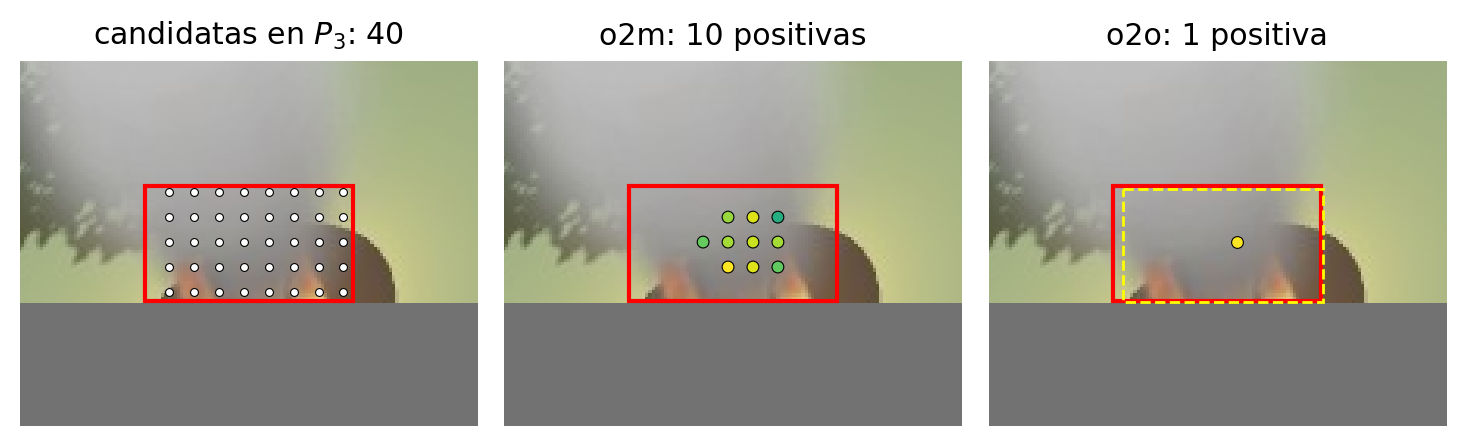
\includegraphics[width=\textwidth]{asignacion.png}
\caption{Asignación real en una imagen de validación con FuegoNet ya entrenada.
Izquierda: celdas candidatas de la caja de fuego (puntos grises) en la escala
$P_3$ (paso 8). Centro: las 10 celdas positivas de la cabeza o2m (color = métrica
$t$). Derecha: la única celda positiva de la o2o y, punteada, la caja que predice.}
\label{fig:asignacion}
\end{figure}

\section{STAL: que ningún foco se quede sin responsable}

Una celda es candidata solo si su \emph{centro} cae dentro de la caja. En la
escala más fina los centros están cada 8 píxeles. Un foco visto desde 60~m puede
medir $6\times5$ píxeles y caer entre cuatro centros sin contener ninguno. Esa
etiqueta queda sin celdas positivas, la red nunca aprende de ella y el error pasa
sin que se note.

STAL (\emph{Small-Target-Aware Label assignment}) resuelve esto. Si un lado de la
caja mide menos que el paso intermedio (16 píxeles), al buscar candidatas se
agranda a 16 píxeles alrededor de su centro. Solo se agranda para elegir
candidatas: el objetivo de la regresión sigue siendo la caja original.

\begin{lstlisting}[style=py]
    def _dentro(self, puntos, cajas):
        c = (cajas[..., :2] + cajas[..., 2:]) / 2
        wh = (cajas[..., 2:] - cajas[..., :2]).clamp(min=self.lado_min)      # STAL
        lt, rb = (c - wh / 2)[:, :, None], (c + wh / 2)[:, :, None]
        d = torch.cat((puntos - lt, rb - puntos), -1)                        # (B, M, A, 4)
        return d.amin(-1) > self.eps
\end{lstlisting}

\section{El código}

\paso{14} \textbf{Escribir \cod{AsignadorTAL}.}
Todo se hace con tensores de forma $(B, M, A)$: imágenes, etiquetas (rellenadas
con ceros hasta el máximo del lote) y celdas. No hay ciclos de Python sobre
celdas ni sobre etiquetas:

\begin{lstlisting}[style=py]
        dentro = self._dentro(puntos, cajas_gt) & valido.bool()              # (B, M, A)
        b, m, a = dentro.nonzero(as_tuple=True)
        iou[b, m, a] = ciou(cajas_gt[b, m], cajas_p[b, a]).clamp_(0)
        s[b, m, a] = prob[b, a, clases_gt[b, m, 0].long()]
        t = s.pow(self.alpha) * iou.pow(self.beta)
        idx = t.topk(self.topk, dim=-1).indices                               # (B, M, k)
        pos = torch.zeros_like(t, dtype=torch.int8).scatter_(-1, idx, 1)
        pos = pos * dentro * valido.to(torch.int8)
        varios = (pos.sum(1, keepdim=True) > 1).expand(-1, M, -1)            # conflictos
        mejor = torch.zeros_like(pos).scatter_(1, iou.argmax(1, keepdim=True), 1)
        pos = torch.where(varios, mejor, pos)
        if self.topk2 != self.topk:                                          # uno a uno
            idx2 = (t * pos).topk(self.topk2, dim=-1).indices
            pos = pos * torch.zeros_like(pos).scatter_(-1, idx2, 1)
\end{lstlisting}

\begin{aviso}
El asignador va decorado con \cod{@torch.no_grad()} y recibe las predicciones
con \cod{.detach()}. La asignación \emph{usa} la predicción para decidir, pero
no se deriva a través de esa decisión. Si se deriva, la red aprende a hacer
trampa con su propia asignación.
\end{aviso}

\begin{ejercicio}
En \cod{perdida.py} cambia \cod{lado_min} a 0 (STAL apagado), entrena 30 épocas y
compara el AP de fuego con el del modelo normal en las imágenes del mundo grande,
donde los focos se ven más pequeños.
\end{ejercicio}

\chapter{La función de pérdida}
\label{cap:perdida}

\begin{enpocas}
Un solo número que diga qué tan mal lo hizo la red: clase, caja y distancias, en
dos cabezas que se combinan con un peso que cambia (ProgLoss). Archivos:
\cod{red_fuego/perdida.py} y \cod{red_fuego/perdida_iou.py}.
\end{enpocas}

\section{Tres términos por cabeza}

Una vez asignadas las celdas, cada cabeza calcula
\begin{equation}
L = 7.5\,L_{\text{caja}} + 0.5\,L_{\text{clase}} + 1.5\,L_{\text{dist}},
\end{equation}
con las ganancias por omisión de Ultralytics. Sea $\Omega$ el conjunto de celdas
positivas, $\hat t_i$ el objetivo suave de la celda $i$
(capítulo~\ref{cap:asignacion}) y $S = \sum_i \hat t_i$.

\subsection{Clase: entropía cruzada binaria}
En \emph{todas} las celdas y para cada clase $c$:
\begin{equation}
L_{\text{clase}} = \frac{1}{S}\sum_{i}\sum_{c} -\big[\hat t_{ic}\log\sigma(z_{ic})
+ (1-\hat t_{ic})\log(1-\sigma(z_{ic}))\big].
\end{equation}
Las celdas de fondo tienen $\hat t = 0$ y aprenden a decir «nada». Se usa una
sigmoide por clase (no un \emph{softmax}) porque fuego y humo pueden aparecer en
la misma celda.

\subsection{Caja: CIoU}
\paso{15} \textbf{Escribir \cod{ciou}.}
El IoU mide el traslape entre la caja predicha $B$ y la real $B^\ast$, pero vale
cero cuando no se tocan y entonces no da gradiente. CIoU (\emph{Complete IoU}) le
resta dos castigos:
\begin{equation}
\mathrm{CIoU} = \mathrm{IoU} - \frac{\rho^2(\mathbf{c},\mathbf{c}^\ast)}{d^2} - \alpha v,
\qquad v = \frac{4}{\pi^2}\Big(\arctan\frac{w^\ast}{h^\ast} - \arctan\frac{w}{h}\Big)^2,
\end{equation}
donde $\rho$ es la distancia entre los centros, $d$ la diagonal de la caja más
pequeña que contiene a las dos y $\alpha = v/(1 - \mathrm{IoU} + v)$. El primer
castigo acerca los centros aunque las cajas no se toquen; el segundo iguala la
proporción ancho/alto. La pérdida es
\begin{equation}
L_{\text{caja}} = \frac{1}{S}\sum_{i\in\Omega}\hat t_i\,\big(1-\mathrm{CIoU}_i\big).
\end{equation}

\subsection{Distancias: L1 (en lugar de DFL)}
Las cuatro distancias $(\ell,t,r,b)$ se comparan directamente con las reales,
pasadas a píxeles y divididas entre el tamaño de la imagen para que todas estén
entre 0 y 1:
\begin{equation}
L_{\text{dist}} = \frac{1}{S}\sum_{i\in\Omega}\hat t_i\;\frac{1}{4}\sum_{k\in\{\ell,t,r,b\}}
\Big|\frac{s_i\,d_{ik}}{640} - \frac{s_i\,d^\ast_{ik}}{640}\Big|.
\end{equation}
Es el término que reemplaza a la DFL de YOLOv8 y YOLO11.

\section{Dos cabezas y ProgLoss}

\paso{16} \textbf{Escribir \cod{PerdidaE2E}.}
La pérdida total combina las dos cabezas:
\begin{equation}
L_{\text{total}} = w(e)\,L_{\text{o2m}} + \big(1 - w(e)\big)\,L_{\text{o2o}},\qquad
w(e) = 0.1 + 0.7\,\Big(1 - \frac{e}{E-1}\Big),
\end{equation}
donde $e$ es la época actual y $E$ el total. Al principio ($w = 0.8$) manda la
cabeza o2m: con diez positivos por objeto, la columna vertebral aprende rápido a
ver fuego. Al final ($w = 0.1$) manda la o2o, que es la que se usará en vuelo.

\begin{figure}[H]
\centering
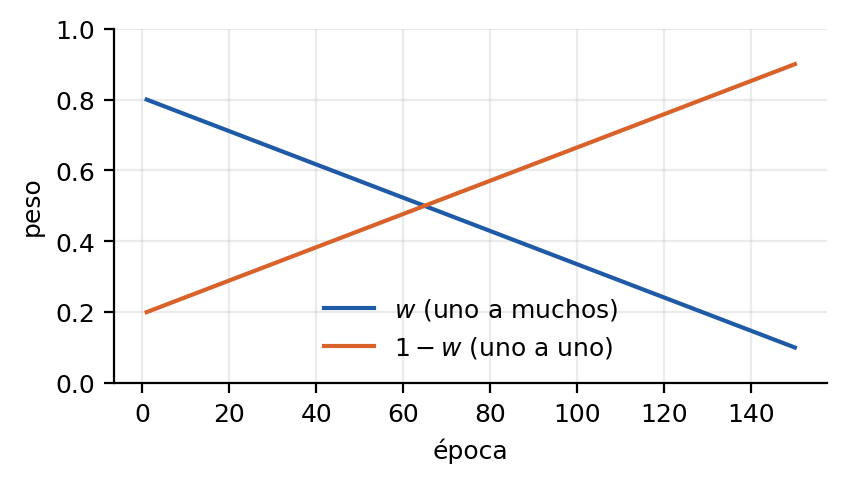
\includegraphics[width=0.62\textwidth]{progloss.png}
\caption{Peso de cada cabeza a lo largo de 150 épocas (ProgLoss).}
\label{fig:progloss}
\end{figure}

\begin{lstlisting}[style=py]
class PerdidaE2E:
    def __init__(self, nc, pasos, epocas, w0=0.8, wf=0.1):
        self.o2m = PerdidaCabeza(nc, pasos, topk=10)
        self.o2o = PerdidaCabeza(nc, pasos, topk=7, topk2=1)
        ...
    def fijar_epoca(self, e):
        self.w = max(1 - e / max(self.epocas - 1, 1), 0) * (self.w0 - self.wf) + self.wf
\end{lstlisting}

\begin{recuerda}
Recuerda el \cod{detach()} de la cabeza (capítulo~\ref{cap:arquitectura}): la
pérdida o2o solo entrena las capas propias de esa cabeza. La columna vertebral y
el cuello los entrena únicamente la o2m. Por eso la o2o puede volverse
«selectiva» sin estorbar a las características que comparten.
\end{recuerda}

\section{Detalles que importan}

\begin{itemize}
  \item La pérdida se calcula en \cod{float32} aunque la red corra en
        \cod{bfloat16} (precisión mixta): los logaritmos y las sumas grandes pierden
        precisión en 16 bits.
  \item Se multiplica por el tamaño del lote $B$ (como Ultralytics) para que la escala
        del gradiente no dependa de $B$ cuando se acumulan lotes.
  \item Si una imagen del lote no tiene objetos, solo contribuye a $L_{\text{clase}}$
        (todo es fondo). Si \emph{ningún} objeto del lote tiene celdas positivas,
        $L_{\text{caja}}$ y $L_{\text{dist}}$ valen cero pero siguen conectadas al
        grafo, así \cod{backward()} no falla.
\end{itemize}

\chapter{Leer los datos y aumentarlos}
\label{cap:datos}

\begin{enpocas}
Cómo se cargan las imágenes y sus etiquetas, cómo se llevan a $640\times640$ sin
deformarlas (letterbox) y qué aumentos se aplican para que 5\,400 imágenes
alcancen. Archivo: \cod{red_fuego/datos.py}.
\end{enpocas}

\section{De archivo a tensor}

\paso{17} \textbf{Escribir \cod{DatasetYolo}.}
Un \cod{Dataset} de PyTorch solo necesita dos métodos: \cod{__len__} (cuántas
muestras hay) y \cod{__getitem__(i)} (dame la muestra $i$). El
\cod{DataLoader} los usa para armar lotes en paralelo con varios procesos
(\cod{num_workers=8}).

Cada muestra devuelve la imagen como tensor \cod{uint8} $(3, 640, 640)$ en RGB y
una tabla de etiquetas $(n, 5)$ con \cod{clase, cx, cy, w, h} normalizados.
La función \cod{juntar} une un lote y agrega a cada etiqueta el índice de su
imagen, porque cada imagen tiene un número distinto de objetos.

\section{Letterbox: cambiar de tamaño sin deformar}

La cámara da $640\times480$ y la red quiere $640\times640$. Estirar la imagen
deformaría las llamas. \textbf{Letterbox} la escala para que el lado mayor mida
640 y rellena el resto con gris (valor 114). Para esta cámara: escala $r = 1$ y
80 píxeles de gris arriba y abajo. Al inferir hay que deshacerlo:
$x_{\text{orig}} = (x - d_x)/r$, $y_{\text{orig}} = (y - d_y)/r$.

\section{Aumentos de datos}

El simulador tiene la luz siempre igual, los mismos árboles y el mismo fuego. Si
la red solo ve eso, aprende detalles que no se repiten en el mundo real (el
\emph{sobreajuste}). Los aumentos crean variantes nuevas en cada época:

\begin{description}
  \item[Mosaico] Cuatro imágenes en un lienzo de $1280\times1280$, alrededor de un
        centro al azar; luego se recorta a $640\times640$. La red ve objetos
        partidos, a varias escalas y con contextos mezclados. Es el aumento que más
        ayuda a YOLO.
  \item[Afín] Escala al azar entre 0.5 y 1.5 y traslación de $\pm10$\,\%. Simula
        volar más alto o más bajo. Las cajas se transforman con la misma matriz y se
        descartan las que quedan casi fuera (menos de 2 píxeles o menos del 10\,\%
        de su área).
  \item[HSV] Tono $\pm1.5$\,\%, saturación $\pm50$\,\% y brillo $\pm40$\,\% con
        tablas de búsqueda (rápido). Simula otra hora del día u otra cámara.
  \item[Espejo] Horizontal con probabilidad 0.5.
\end{description}

\paso{18} \textbf{Ver los aumentos antes de entrenar.}
Este es el paso más importante del capítulo: si las cajas no coinciden con el
fuego después de aumentar, la red aprende basura y el error no aparece en ningún
lado.

\begin{lstlisting}[style=py]
from cuadrirotor_sim.red_fuego.datos import DatasetYolo
ds = DatasetYolo('.../data.yaml', 'train', 640, aumentar=True)
img, e = ds[3000]                     # dibuja e sobre img y guárdala
\end{lstlisting}

\begin{figure}[H]
\centering
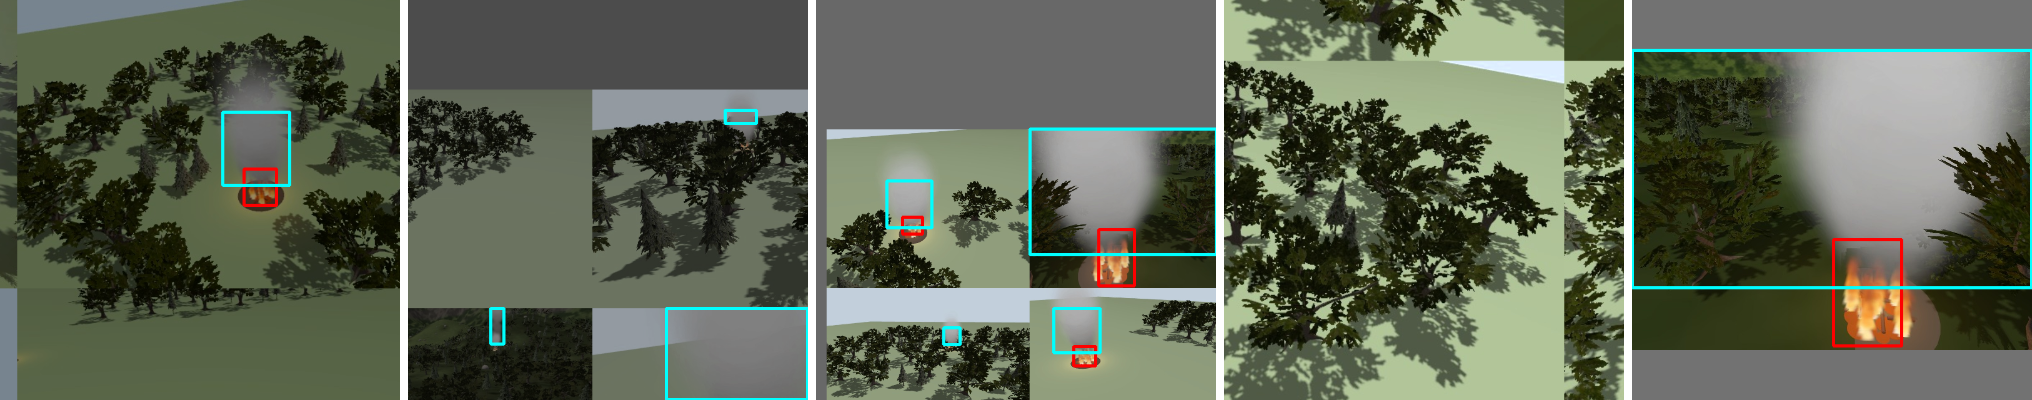
\includegraphics[width=\textwidth]{aumentos.png}
\caption{Cuatro muestras aumentadas (mosaico + afín + HSV + espejo) y una de
validación sin aumentar (derecha). Rojo: fuego. Cian: humo.}
\label{fig:aumentos}
\end{figure}

\begin{resultado}
Cada caja roja encierra llamas y cada caja cian una columna de humo, incluso en
los pedazos del mosaico. Las franjas grises son el relleno.
\end{resultado}

\begin{consejo}
En las últimas 10 épocas se apaga el mosaico (\cod{--sin-mosaico 10}). Así la
red termina viendo imágenes como las que verá en vuelo. Como los procesos del
\cod{DataLoader} guardan su propia copia del dataset, al cambiar
\cod{ds.mosaico} hay que crear un \cod{DataLoader} nuevo.
\end{consejo}

\begin{leccion}
Las etiquetas de las imágenes sin fuego son archivos vacíos y
\cod{np.loadtxt} da un aviso por cada uno (más de mil líneas en la terminal). Se
revisa el tamaño del archivo antes de leerlo:
\begin{lstlisting}[style=py]
    if not os.path.exists(p) or os.path.getsize(p) == 0:   # imagen sin fuego ni humo
        return np.zeros((0, 5), np.float32)
\end{lstlisting}
\end{leccion}

\chapter{Entrenar}
\label{cap:entrenar}

\begin{enpocas}
El optimizador MuSGD, la tasa de aprendizaje con calentamiento, el promedio móvil
de pesos (EMA) y el ciclo que junta todo. Al final, el comando para entrenar
FuegoNet-n desde cero y lo que pasó en las 150 épocas. Archivos:
\cod{red_fuego/optimizador.py} y \cod{red_fuego/entrenar.py}.
\end{enpocas}

\section{El optimizador MuSGD}

Entrenar es repetir: calcular la pérdida de un lote, obtener el gradiente
$\mathbf{g} = \nabla L$ con \cod{backward()} y mover los pesos un poco en
contra. El descenso por gradiente estocástico con momento (SGD) hace
\begin{equation}
\mathbf{m} \leftarrow \mu\,\mathbf{m} + \mathbf{g},\qquad
\mathbf{W} \leftarrow \mathbf{W} - \eta\,(\mathbf{g} + \mu\,\mathbf{m})\quad\text{(Nesterov)}.
\end{equation}

\textbf{Muon} trata cada matriz de pesos como un todo. Una convolución
$c_{\text{out}}\times c_{\text{in}}\times k\times k$ se ve como matriz
$\mathbf{G}$ de $c_{\text{out}}\times(c_{\text{in}}k^2)$. Si
$\mathbf{G} = \mathbf{U}\mathbf{S}\mathbf{V}^\top$ (descomposición en valores
singulares), Muon cambia la actualización por $\mathbf{U}\mathbf{V}^\top$: la
misma dirección, pero con \emph{todos} los valores singulares iguales a 1. Ninguna
dirección domina a las demás y las «débiles» también avanzan.

Calcular la SVD en cada paso sería lentísimo. Muon aproxima
$\mathbf{U}\mathbf{V}^\top$ con cinco iteraciones de Newton-Schulz, solo con
multiplicaciones de matrices:
\begin{equation}
\mathbf{X}_0 = \frac{\mathbf{G}}{\|\mathbf{G}\|_F},\qquad
\mathbf{A} = \mathbf{X}\mathbf{X}^\top,\qquad
\mathbf{X} \leftarrow a\,\mathbf{X} + (b\,\mathbf{A} + c\,\mathbf{A}^2)\,\mathbf{X},
\end{equation}
con $a = 3.4445$, $b = -4.7750$ y $c = 2.0315$.

\paso{19} \textbf{Escribir \cod{ortogonalizar} y \cod{MuSGD}.}
\begin{lstlisting}[style=py]
def ortogonalizar(G, pasos=5, eps=1e-7):
    a, b, c = 3.4445, -4.7750, 2.0315
    X = G.bfloat16()
    X = X / (X.norm() + eps)                 # valor singular mayor <= 1
    alta = G.size(0) > G.size(1)
    if alta:
        X = X.T
    for _ in range(pasos):
        A = X @ X.T
        X = a * X + (b * A + c * A @ A) @ X
    return (X.T if alta else X).to(G.dtype)
\end{lstlisting}

YOLO26 aplica a los pesos de convolución las \emph{dos} actualizaciones, Muon con
factor 0.2 y SGD con factor 1:
\begin{equation}
\mathbf{W} \leftarrow \mathbf{W} - 0.2\,\eta\,\mathrm{Muon}(\mathbf{g})
\sqrt{\max(1, c_{\text{out}}/c_{\text{in}}k^2)}
- \eta\,\mathrm{SGD}(\mathbf{g} + \lambda\mathbf{W}),
\end{equation}
y a los sesgos y a BatchNorm solo SGD, sin decaimiento de pesos ($\lambda = 0$).

\section{Tasa de aprendizaje, calentamiento y lote nominal}

\begin{itemize}
  \item \textbf{Ley lineal}: $\eta(e) = \eta_0\,[(1 - e/E)(1 - 0.01) + 0.01]$, de
        $\eta_0 = 0.01$ a $0.0001$.
  \item \textbf{Calentamiento}: en las primeras 3 épocas $\eta$ sube desde 0 (los
        sesgos bajan desde 0.1) y el momento de 0.8 a 0.9. Con pesos al azar, un paso
        grande al principio puede arruinar las estadísticas de BatchNorm.
  \item \textbf{Lote nominal 64}: con lotes de 32 se acumulan dos gradientes antes de
        cada paso. El decaimiento de pesos se escala por $32\cdot2/64 = 1$.
  \item \textbf{Recorte}: la norma del gradiente se limita a 10.
\end{itemize}

\section{EMA: el modelo suavizado}

Se guarda una copia de la red cuyos pesos son un promedio móvil exponencial de
los pesos de entrenamiento:
\begin{equation}
\mathbf{W}_{\text{EMA}} \leftarrow d\,\mathbf{W}_{\text{EMA}} + (1-d)\,\mathbf{W},\qquad
d = 0.9999\,\big(1 - e^{-n/2000}\big),
\end{equation}
donde $n$ es el número de pasos dados. La EMA ignora el «temblor» de cada lote. Es
la que se valida y se guarda.

\section{El ciclo de entrenamiento}

\paso{20} \textbf{Escribir el ciclo.}
Lo esencial de \cod{entrenar.py}:
\begin{lstlisting}[style=py]
for epoca in range(a.epocas):
    perdida.fijar_epoca(epoca)                     # ProgLoss
    for k, lote in enumerate(carga_ent):
        ...                                        # calentamiento de lr y momento
        lote['img'] = lote['img'].to(disp).float() / 255
        with torch.autocast('cuda', torch.bfloat16):
            pred = modelo(lote['img'])             # {'o2m': ..., 'o2o': ...}
        l, partes = perdida(pred, lote)
        (l / acumular).backward()
        if (k + 1) % acumular == 0:
            torch.nn.utils.clip_grad_norm_(modelo.parameters(), 10.0)
            opt.step(); opt.zero_grad(set_to_none=True)
            ema.actualizar(modelo)
    m = validar(ema.m, carga_val, nc, disp)        # mAP en las 600 de validación
    # guarda ultimo.pt y, si 0.1 mAP50 + 0.9 mAP50-95 mejoró, mejor.pt
\end{lstlisting}

\begin{nota}
\cod{torch.autocast} con \cod{bfloat16} hace las convoluciones en 16 bits (más
rápido, la mitad de memoria) y deja en 32 bits lo delicado. A diferencia de
\cod{float16}, \cod{bfloat16} tiene el mismo rango que \cod{float32}, así que no
necesita \cod{GradScaler}. Las tarjetas RTX de la serie 30 en adelante lo
soportan.
\end{nota}

\paso{21} \textbf{Primera prueba: tres épocas.}
Antes de lanzar horas de entrenamiento se corre una prueba corta. Si hay un error
en la asignación o en la pérdida, el mAP se queda en cero:
\begin{lstlisting}[style=bash]
~/.venvs/yolo/bin/python -m cuadrirotor_sim.red_fuego.entrenar \
  --datos ~/datasets/combinado_incendio_bosque_incendio_bosque_grande/data.yaml \
  --epocas 3 --salida /tmp/prueba_fuegonet
\end{lstlisting}
\begin{resultado}
\begin{lstlisting}
FuegoNet-n: 2.50 M parámetros, 5400 imágenes de entrenamiento, 600 de validación
[  1/3] pérdida caja 3.364 clase 8.700 dist 0.045 | mAP50 0.001 mAP50-95 0.000 | 74 s
[  2/3] pérdida caja 3.004 clase 4.437 dist 0.042 | mAP50 0.077 mAP50-95 0.022 | 122 s
[  3/3] pérdida caja 2.507 clase 2.656 dist 0.034 | mAP50 0.512 mAP50-95 0.198 | 171 s
\end{lstlisting}
Las tres pérdidas bajan y el mAP50 sube de 0 a 0.5 en tres épocas, sin ningún
peso preentrenado. La red está aprendiendo.
\end{resultado}

\paso{22} \textbf{Entrenamiento completo.}
\begin{lstlisting}[style=bash]
nohup ~/.venvs/yolo/bin/python -m cuadrirotor_sim.red_fuego.entrenar \
  --datos ~/datasets/combinado_incendio_bosque_incendio_bosque_grande/data.yaml \
  --epocas 150 --salida ~/datasets/fuegonet/n_150 > ~/datasets/fuegonet/n_150.log 2>&1 &
tail -f ~/datasets/fuegonet/n_150.log
\end{lstlisting}
Cada época queda en una fila de \cod{resultados.csv}: tiempo, las tres pérdidas
de la o2o, P, R, mAP50, mAP50-95, AP por clase, tasa de aprendizaje y peso $w$
de ProgLoss.

\section{Qué pasó en el entrenamiento}

\begin{figure}[H]
\centering
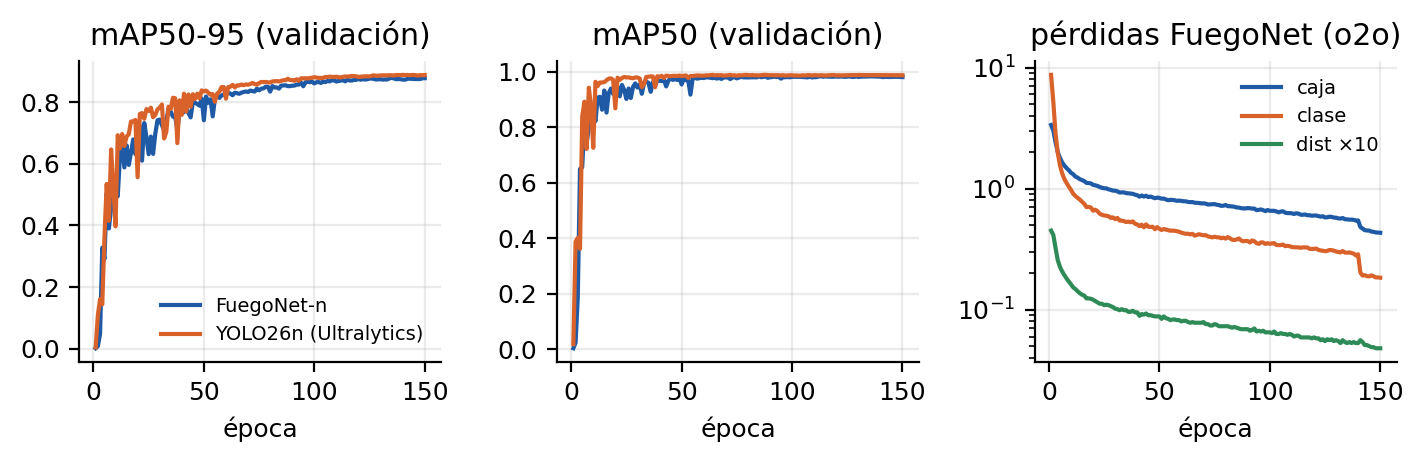
\includegraphics[width=\textwidth]{curvas.png}
\caption{Entrenamiento desde cero. Izquierda y centro: mAP en validación de
FuegoNet-n (este manual) y de YOLO26n de Ultralytics con la misma receta.
Derecha: pérdidas de la cabeza o2o de FuegoNet (escala logarítmica).}
\label{fig:curvas}
\end{figure}

\begin{itemize}
  \item El entrenamiento corrió 150 épocas en 156 minutos
        (unos 62~s por época, compartiendo la
        GPU con la corrida de control).
  \item El mejor modelo (\cod{mejor.pt}) es el de la época 135: mAP50 =
        0.984 y mAP50-95 = 0.879 en validación
        (AP50-95 de fuego 0.879, de humo 0.879).
  \item En la época 10 ya tenía mAP50 = 0.859: la mayor parte se aprende
        pronto y las últimas épocas afinan las cajas (sube sobre todo el mAP50-95).
  \item Al apagar el mosaico (últimas 10 épocas) hay un salto pequeño hacia arriba: la
        red se ajusta a imágenes completas como las de vuelo.
\end{itemize}

\begin{nota}
La curva naranja es el control: YOLO26n de Ultralytics, también desde cero, con los
mismos datos y aumentos. Su mejor época (140) da mAP50-95 =
0.889 \emph{según su propio validador}. La comparación
justa, con el mismo código de métricas, está en el capítulo~\ref{cap:evaluar}.
\end{nota}



\part{Medir y usar la red}
\chapter{Medir y comparar con YOLO26n}
\label{cap:evaluar}

\begin{enpocas}
Cómo se calcula el mAP, por qué hay que medir todas las redes con el mismo
código y cómo queda FuegoNet-n frente a YOLO26n entrenado desde cero y frente al
YOLO26n preentrenado que usa hoy la simulación. Archivos:
\cod{red_fuego/metricas.py} y \cod{red_fuego/evaluar.py}.
\end{enpocas}

\section{mAP en pocas palabras}

Para un umbral de traslape $\tau$, una predicción es un \textbf{verdadero
positivo} si su IoU con una etiqueta de su misma clase es $\ge\tau$ y esa
etiqueta no la tomó antes otra predicción con más confianza. Ordenando todas las
predicciones de la clase por confianza se obtienen la precisión
$P = \text{VP}/(\text{VP}+\text{FP})$ y la exhaustividad (\emph{recall})
$R = \text{VP}/N_{\text{etiquetas}}$ para cada corte. El \textbf{AP} es el área
bajo la curva $P(R)$ (con su envolvente decreciente, integrada en 101 puntos,
como COCO).
\begin{itemize}
  \item \textbf{mAP50}: AP con $\tau = 0.5$, promediado en las dos clases. ¿Encontró el fuego?
  \item \textbf{mAP50-95}: promedio en $\tau = 0.50, 0.55,\dots,0.95$. ¿Qué tan
        ajustada está la caja? Es la métrica principal.
\end{itemize}

\paso{23} \textbf{Escribir el acumulador de métricas.}
\cod{Acumulador.agregar(pred, gt)} recibe, imagen por imagen, las predicciones
$(N,6)$ y las etiquetas $(M,5)$, y guarda qué predicciones fueron VP en cada uno de
los 10 umbrales. \cod{calcular()} ordena todo por confianza y devuelve mAP50,
mAP50-95, AP por clase, y P y R con confianza $\ge 0.25$ (el umbral del
detector en vuelo).

\begin{aviso}
Ultralytics reporta su propio mAP, pero calcula la validación con imágenes
rectangulares agrupadas, su propio emparejamiento y su propio preprocesamiento.
Comparar su número con el nuestro sería comparar dos reglas distintas.
\cod{evaluar.py} corre las \emph{tres} redes sobre las mismas 600 imágenes
originales ($640\times480$), con umbral de confianza $0.001$ y hasta 300
detecciones, y las mide con el \emph{mismo} \cod{Acumulador}.
\end{aviso}

\section{Las tres redes que se comparan}

\begin{description}
  \item[FuegoNet-n] nuestra red, desde cero, 150 épocas (capítulo~\ref{cap:entrenar}).
  \item[YOLO26n desde cero] la red de Ultralytics con la misma arquitectura
        (\cod{yolo26n.yaml}, \cod{pretrained=False}), los mismos datos, aumentos y
        épocas. Es el \textbf{control}: si nuestro código está bien, debe salir
        parecida a FuegoNet-n.
  \item[YOLO26n preentrenado] el de la simulación (\cod{yolo/incendio_yolo26n.pt}):
        pesos de COCO ajustados 60 épocas a fuego y humo.
\end{description}

\paso{24} \textbf{Correr la evaluación.}
\begin{lstlisting}[style=bash]
~/.venvs/yolo/bin/python -m cuadrirotor_sim.red_fuego.evaluar \
  --datos ~/datasets/combinado_incendio_bosque_incendio_bosque_grande/data.yaml \
  --fuegonet ~/datasets/fuegonet/n_150/mejor.pt \
  --yolo ~/datasets/fuegonet/yolo26n_desde_cero/weights/best.pt yolo/incendio_yolo26n.pt \
  --salida ~/datasets/fuegonet/evaluacion.json
\end{lstlisting}

\section{Resultados}

\begin{table}[H]
\centering\scriptsize
\setlength{\tabcolsep}{3.5pt}
\caption{Las tres redes medidas con el mismo código sobre las 600 imágenes de
validación. P y R con confianza $\ge0.25$ e IoU 0.5. Mediana de la latencia por imagen (lote 1,
incluye pre y posprocesamiento) en la RTX~5060~Ti y en CPU con 4 hilos.}
\label{tab:comparacion}
\resizebox{\textwidth}{!}{%
\begin{tabular}{lrrrrrrrrrr}
\toprule
\textbf{Red} & \textbf{Parám.\ (M)} & \textbf{GFLOPs} & \textbf{P} & \textbf{R} &
\textbf{mAP50} & \textbf{mAP50-95} & \textbf{AP fuego} & \textbf{AP humo} &
\textbf{GPU (ms)} & \textbf{CPU (ms)}\\
\midrule
FuegoNet-n & 2.50 & 5.3 & 0.918 & 0.971 & 0.984 & 0.899 & 0.912 & 0.886 & 4.0 & 32.6 \\
YOLO26n desde cero & 2.50 & 5.7 & 0.893 & 0.981 & 0.984 & 0.888 & 0.904 & 0.872 & 3.8 & 15.5 \\
YOLO26n preentrenado (COCO) & 2.53 & 5.9 & 0.912 & 0.973 & 0.984 & 0.881 & 0.895 & 0.867 & 4.0 & 21.1 \\
\bottomrule
\end{tabular}}
\end{table}

\paragraph{FuegoNet-n contra YOLO26n desde cero.} Es la comparación que valida
el código: misma arquitectura, mismos datos, mismas épocas y sin preentrenamiento.
Las dos tienen los mismos 2.505~M de parámetros: es la misma red.
FuegoNet-n hace 5.3~GFLOPs y no 5.7 porque al inferir ya no
calcula la cabeza o2m, que Ultralytics sí calcula aunque no la use. FuegoNet-n queda
por encima en 0.011 de mAP50-95
(0.899 contra 0.888). Es una sola corrida de cada una:
para decir que una es mejor habría que repetir con varias semillas. Lo que sí se
puede concluir es que la red propia \emph{reproduce} a YOLO26n. Además, el
validador de Ultralytics le da 0.889 a su modelo y nuestro código
0.888, así que también el código de métricas coincide.

\paragraph{Contra el YOLO26n preentrenado.} El modelo que usa hoy la simulación da
mAP50-95 = 0.881, 0.018 por debajo de
FuegoNet-n. Puede sorprender, porque partió de pesos de COCO (118\,000 imágenes).
Pero se ajustó solo 60 épocas y FuegoNet entrenó 150, y las imágenes de validación
vienen del mismo simulador que las de entrenamiento. En este caso, más épocas sobre
datos del dominio pesan más que el preentrenamiento. Con imágenes reales de
incendios, donde COCO sí aporta, el resultado podría invertirse
(capítulo~\ref{cap:siguientes}). En mAP50 las tres redes empatan
(0.984): todas encuentran el fuego. La diferencia está en qué tan
ajustadas quedan las cajas.

\paragraph{Velocidad.} En la GPU las tres tardan entre 4
y 4~ms por imagen (mediana de 100), contando el
pre y el posprocesamiento: unas 250 imágenes por segundo. En CPU, FuegoNet-n tarda
33~ms y los YOLO26n entre 16 y
21~ms. Aunque es la misma red, Ultralytics infiere con
la imagen \emph{rectangular} de $640\times480$ y FuegoNet con el cuadrado de
$640\times640$ (25\,\% más píxeles). Con \cod{Detector(..., rect=True)} FuegoNet
baja a unos 23~ms, pero su mAP50-95 cae de 0.899 a 0.886 porque se entrenó solo con
imágenes cuadradas. Por eso, por omisión, se usa el cuadrado. Los tiempos en CPU
varían algunos milisegundos de una medición a otra.

\begin{leccion}
Durante el entrenamiento, el mejor modelo (época 135) marcaba mAP50-95 =
0.879 y aquí da 0.899. La diferencia viene de la precisión:
\cod{entrenar.py} valida con \cod{bfloat16} (rápido) y \cod{evaluar.py} en
\cod{float32}. Con 8 bits de mantisa, una coordenada entre 512 y 1024 píxeles se
redondea de 4 en 4 píxeles, y eso castiga los umbrales de IoU altos (0.90, 0.95).
Se comprobó validando el mismo \cod{mejor.pt} de las dos formas: 0.880 en
\cod{bfloat16} y 0.898 en \cod{float32}. Para reportar resultados,
usa siempre \cod{evaluar.py}. Queda pendiente decodificar las cajas en
\cod{float32} dentro de \cod{Cabeza.decodificar}: así la elección del mejor
modelo también usaría la métrica exacta.
\end{leccion}

\begin{figure}[H]
\centering
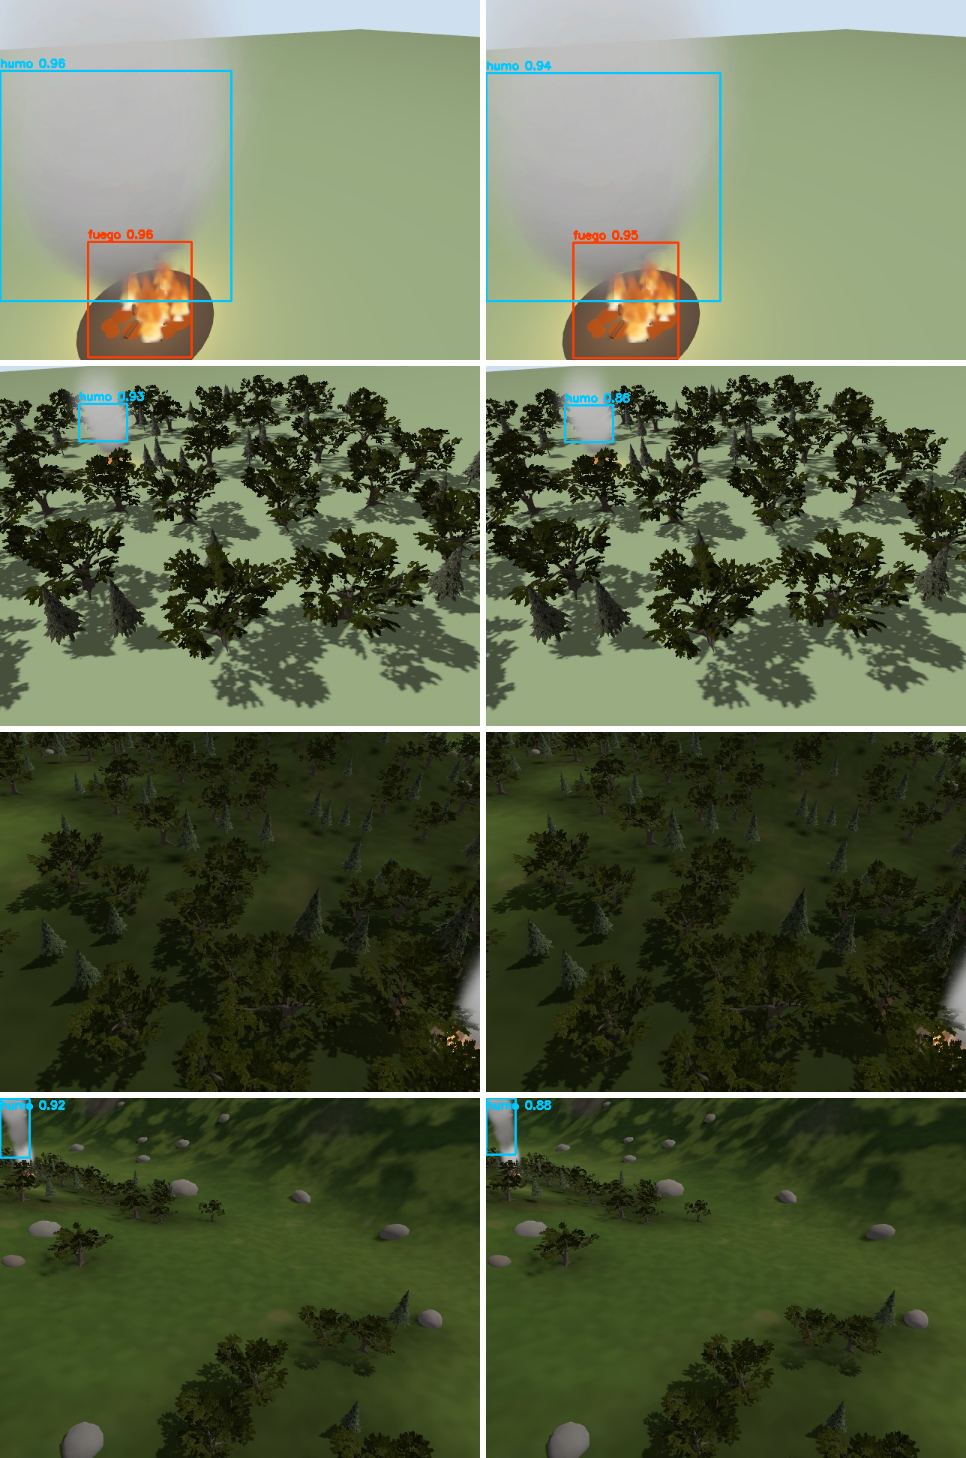
\includegraphics[width=0.92\textwidth]{detecciones.png}
\caption{Detecciones con confianza $\ge 0.25$ en cuatro imágenes de validación.
Izquierda: FuegoNet-n (sin NMS). Derecha: YOLO26n preentrenado de la simulación.}
\label{fig:detecciones}
\end{figure}


\chapter{Usar la red: imágenes, ONNX y ROS 2}
\label{cap:integrar}

\begin{enpocas}
Detectar en una foto, exportar la red a ONNX para la computadora a bordo y
conectarla a la simulación para que el Tarot 650 busque el incendio con
FuegoNet. Archivos: \cod{red_fuego/inferir.py}, \cod{red_fuego/exportar.py},
\cod{detector_yolo.py} y \cod{launch/simulacion.launch.py}.
\end{enpocas}

\section{Detectar en una imagen}

\paso{25} \textbf{Probar el detector.}
La clase \cod{Detector} carga \cod{mejor.pt}, aplica letterbox, corre la red,
aplica el umbral de confianza (no hay NMS) y regresa las cajas a las coordenadas
de la imagen original.

Al cargar los pesos, \cod{fusionar} pliega cada BatchNorm en su convolución.
Al inferir, BatchNorm es solo una transformación lineal fija por canal:
\begin{equation}
y = \gamma\,\frac{W x - \mu}{\sqrt{\sigma^2+\epsilon}} + \beta
  = \underbrace{\frac{\gamma}{\sqrt{\sigma^2+\epsilon}}W}_{W'}\,x
  + \underbrace{\beta - \frac{\gamma\,\mu}{\sqrt{\sigma^2+\epsilon}}}_{b'},
\end{equation}
así que se puede meter dentro de los pesos de la convolución. Da exactamente las
mismas cajas (el mAP no cambia) con una operación menos por capa.

\begin{lstlisting}[style=bash]
~/.venvs/yolo/bin/python -m cuadrirotor_sim.red_fuego.inferir \
  ~/datasets/fuegonet/n_150/mejor.pt ~/datasets/incendio_bosque/images/val/00420.jpg salida.jpg
\end{lstlisting}

\begin{resultado}
\begin{lstlisting}
2 detecciones en 6.1 ms
  fuego  0.96  caja 117.2 322.9 255.2 476.0
  humo   0.96  caja 0.0 94.8 308.8 401.7
\end{lstlisting}
Cada fila es una caja: clase, confianza y $(x_1, y_1, x_2, y_2)$ en píxeles de la imagen
original de $640\times480$.
\end{resultado}


\section{Exportar a ONNX}

ONNX es un formato abierto que entienden TensorRT (Jetson), OpenVINO (Intel),
ONNX Runtime (cualquier CPU) y muchos otros. Como FuegoNet no tiene NMS, todo el
detector cabe en el grafo y la salida es un solo tensor $(1, 300, 6)$.

\paso{26} \textbf{Instalar \cod{onnx} sin romper NumPy.}
\begin{lstlisting}[style=bash]
~/.venvs/yolo/bin/pip install onnx onnxruntime
~/.venvs/yolo/bin/pip install "numpy==1.26.4" "ml-dtypes<0.6"   # ¡regresar NumPy!
\end{lstlisting}

\begin{leccion}
Al instalar \cod{onnx}, pip subió NumPy de 1.26 a 2.5 y \cod{ml-dtypes} a una
versión que exige NumPy~2. ROS 2 Jazzy está compilado contra NumPy~1 y el nodo
detector habría dejado de arrancar. La segunda línea regresa NumPy y fija una
\cod{ml-dtypes} compatible. Comprueba siempre con
\cod{python -c "import numpy; print(numpy.__version__)"} después de instalar algo.
\end{leccion}

\paso{27} \textbf{Exportar y comprobar.}
\begin{lstlisting}[style=bash]
~/.venvs/yolo/bin/python -m cuadrirotor_sim.red_fuego.exportar \
  ~/datasets/fuegonet/n_150/mejor.pt ~/datasets/fuegonet/fuegonet_n.onnx \
  ~/datasets/incendio_bosque/images/val/00420.jpg
\end{lstlisting}
El tercer argumento es una foto para comprobar que ONNX Runtime y PyTorch dan las
mismas detecciones.
\begin{resultado}
\begin{lstlisting}
Exportado /home/jairo/datasets/fuegonet/fuegonet_n.onnx
2 detecciones con confianza >= 0.25; diferencia máxima ONNX vs PyTorch: 3.05e-05
\end{lstlisting}
El archivo pesa 9.6~MB. La entrada se llama \cod{imagen} $(1,3,640,640)$ y la
salida \cod{detecciones} $(1,300,6)$.
\end{resultado}


\begin{leccion}
La primera comprobación usaba una entrada de ruido y comparaba las 300 filas. Daba
diferencias de más de 500 píxeles. No era un error de exportación: con ruido casi
todas las confianzas son $\approx 0$ y están empatadas, y \cod{topk} las ordena
distinto en PyTorch y en ONNX Runtime, así que se comparaban cajas de celdas
distintas. Ahora se usa una foto real y solo las detecciones con confianza
$\ge 0.25$. La diferencia baja a $3\times10^{-5}$ píxeles.
\end{leccion}

\section{Conectar FuegoNet a la simulación}

El nodo \cod{detector_yolo} ya publicaba \cod{/cuadrirotor/detecciones}
(\cod{vision_msgs/Detection2DArray}) con YOLO26 de Ultralytics. Para no duplicar
el nodo, \cod{inferir.py} incluye una envoltura \cod{ComoYolo} con la misma
interfaz que usa el nodo (\cod{.names} y \cod{.predict(...)[0].boxes}). El nodo
elige según la terminación del archivo de pesos:

\begin{lstlisting}[style=py]
        if v['modelo'].endswith('.fuegonet.pt'):
            from cuadrirotor_sim.red_fuego.inferir import ComoYolo
            self.modelo, self.etiqueta = ComoYolo(v['modelo'], v['dispositivo']), 'FuegoNet'
        else:
            self.modelo, self.etiqueta = YOLO(v['modelo']), 'YOLO26'
\end{lstlisting}

\paso{28} \textbf{Instalar los pesos en el paquete.}
\begin{lstlisting}[style=bash]
cp ~/datasets/fuegonet/n_150/mejor.pt \
   ~/ros2_ws/src/cuadrirotor_sim/yolo/incendio_fuegonet_n.fuegonet.pt
cd ~/ros2_ws && colcon build --packages-select cuadrirotor_sim --symlink-install
source install/setup.bash
\end{lstlisting}

\paso{29} \textbf{Volar la búsqueda con FuegoNet.}
El \emph{launch} tiene un argumento nuevo, \cod{red}, que elige el detector
(\cod{yolo26}, el de siempre, o \cod{fuegonet}):
\begin{lstlisting}[style=bash]
ros2 launch cuadrirotor_sim simulacion.launch.py mision:=busqueda red:=fuegonet
\end{lstlisting}
\begin{resultado}
En la terminal aparece \cod{YOLO listo: incendio_fuegonet_n.fuegonet.pt, clases
\{0: 'fuego', 1: 'humo'\}} y el panel «Detección YOLO» de Gazebo muestra
\cod{FuegoNet  xx ms} en la esquina. El resto de la misión (barrido, verificación,
aviso GPS) no cambia, porque los mensajes son los mismos.
\end{resultado}

\begin{consejo}
Para comparar las dos redes en las mismas condiciones, corre la misión dos veces
con el mismo \cod{mundo}, \cod{foco_x}, \cod{foco_y} y \cod{viento}, una con
\cod{red:=yolo26} y otra con \cod{red:=fuegonet}, y compara el tiempo hasta la
confirmación y las falsas alarmas.
\end{consejo}

\chapter{Qué sigue}
\label{cap:siguientes}

\begin{enpocas}
Resumen de lo construido, cómo reportarlo en un artículo o reporte y experimentos que valen la
pena con FuegoNet.
\end{enpocas}

\section{Lo que ya tienes}

\begin{itemize}
  \item Una implementación propia, legible y sin dependencias externas de la
        arquitectura y la receta de entrenamiento de YOLO26: bloques C3k2, SPPF y
        C2PSA, cabeza sin DFL ni NMS, TAL con STAL, pérdida de dos cabezas con
        ProgLoss y optimizador MuSGD.
  \item Un modelo entrenado desde cero, medido con un protocolo propio y
        comparado contra la implementación de referencia.
  \item La red conectada a la misión de búsqueda (\cod{red:=fuegonet}) y exportable
        a ONNX.
\end{itemize}

\section{Cómo reportarlo}

\begin{enumerate}
  \item En el marco teórico, describe la arquitectura con la
        figura~\ref{fig:arquitectura} y la tabla~\ref{tab:capas}, y la asignación y la
        pérdida con las ecuaciones de los capítulos~\ref{cap:asignacion}
        y~\ref{cap:perdida}.
  \item En la metodología, da el dataset (tabla~\ref{tab:dataset}), los aumentos, los
        hiperparámetros del capítulo~\ref{cap:entrenar} y el protocolo de medición
        (mismo código para todas las redes).
  \item En los resultados, la tabla comparativa del capítulo~\ref{cap:evaluar} y las
        curvas de entrenamiento. Separa con claridad «arquitectura igual» de «pesos
        iniciales distintos».
  \item Cita YOLO26 por su documentación de Ultralytics, YOLOv10 por la idea de la
        doble asignación sin NMS, TOOD por TAL y el trabajo de Muon por el optimizador.
\end{enumerate}

\section{Experimentos sugeridos}

\begin{description}
  \item[Ablación] Quitar una pieza a la vez y medir: sin STAL (\cod{lado_min=0}),
        sin atención (\cod{atencion=False} en \cod{h22} y sin \cod{C2PSA}), SGD en
        lugar de MuSGD (\cod{--optimizador sgd}), sin ProgLoss ($w$ fijo en 0.5). Cada
        pieza debe justificar su lugar.
  \item[Escala] Entrenar FuegoNet-s (\cod{--escala s}, 10~M parámetros) y ver si el
        aumento de mAP compensa la latencia en la computadora a bordo.
  \item[Preentrenamiento propio] Entrenar primero con un dataset público de incendios
        reales (por ejemplo D-Fire) y después ajustar con el simulador. En el simulador
        FuegoNet ya supera al YOLO26n preentrenado, pero con imágenes reales el
        preentrenamiento suele pesar mucho más.
  \item[Varias semillas] Repetir FuegoNet-n y el YOLO26n desde cero con 3 semillas
        (\cod{--semilla}) y reportar media y desviación. Solo así se puede afirmar que
        una diferencia de 0.01 en mAP50-95 es real.
  \item[Fusionar BatchNorm] Plegar cada BatchNorm en su convolución y quitar la cabeza
        o2m antes de inferir, para acercar la latencia en CPU a la de Ultralytics.
  \item[Del simulador al mundo real] Probar la red con videos reales de incendios
        tomados con dron. Ahí se verá si los aumentos de color alcanzan o si hace
        falta aleatorizar más el simulador (texturas, luz, niebla).
  \item[Clase «distractor»] Agregar una tercera clase para lo que hoy da falsas
        alarmas (rocas oscuras, claros con sol) en lugar de dejarlo como fondo.
\end{description}

\begin{recuerda}
Una red que mide bien en validación todavía no está probada en vuelo. La prueba
final es la misión completa: cuánto tarda el Tarot 650 en encontrar y confirmar
el foco, y cuántas falsas alarmas da en el camino.
\end{recuerda}


\appendix
\chapter{Código completo}
\label{ap:codigo}

Estos son los archivos de \cod{cuadrirotor_sim/red_fuego/} tal como se usaron
para los resultados de este manual.

\section{\texttt{bloques.py}}
\lstinputlisting[style=py]{codigo/bloques.py}
\section{\texttt{modelo.py}}
\lstinputlisting[style=py]{codigo/modelo.py}
\section{\texttt{asignador.py}}
\lstinputlisting[style=py]{codigo/asignador.py}
\section{\texttt{perdida\_iou.py}}
\lstinputlisting[style=py]{codigo/perdida_iou.py}
\section{\texttt{perdida.py}}
\lstinputlisting[style=py]{codigo/perdida.py}
\section{\texttt{datos.py}}
\lstinputlisting[style=py]{codigo/datos.py}
\section{\texttt{optimizador.py}}
\lstinputlisting[style=py]{codigo/optimizador.py}
\section{\texttt{entrenar.py}}
\lstinputlisting[style=py]{codigo/entrenar.py}
\section{\texttt{metricas.py}}
\lstinputlisting[style=py]{codigo/metricas.py}
\section{\texttt{evaluar.py}}
\lstinputlisting[style=py]{codigo/evaluar.py}
\section{\texttt{inferir.py}}
\lstinputlisting[style=py]{codigo/inferir.py}
\section{\texttt{exportar.py}}
\lstinputlisting[style=py]{codigo/exportar.py}


\end{document}
